\documentclass[../main.tex]{subfiles}

\begin{document}

\subsection{External interfaces requirements}

\subsubsection{User interfaces}

The mobile application was designed taking into account that users can utilize only the core functionality of the app (Track4Help) or all services offered (track4Run \& AutomatedSOS).\\
Opening the application, user is presented with the login page (Fig. 8.a), if not already registered, he can sign in.\\
 Once logged in the user is presented with his "Main Feed" (Fig. 8.b), in this page all important information (upcoming runs, smartdevices status and company requests) are presented in a scroll page with clickable panels,
  the objective is to aggregate all three services informations in one screen to simplify the UX.
 At the bottom of the screen a navigation bar makes possible to navigate application's pages.\\
 The user devices page (Fig 9.a) show all user devices, the user can remove a device clicking on the "X" next to the device or add one clicking on the "+" button.
 It's impossible to remove a device if it is associated with AutomatedSOS, the user need to disable AutomatedSOS on that device first.\\
 The AutomatedSOS page (Fig. 9.b) show the status of the devices and lifesign readings. In the example one device is offline and marked with a warning red color.
 Here user can add or disable AutomatedSOS on his owned devices.\\
By clicking on Sharing in the settings screen (Fig 10.a) the user is presented with the sharing page (Fig 10.b), here he can visualize approved and pending requests from companies.\\
 The run page (Fig 11.a) shows all available runs in the users vicinity. It also shows the subscribed runs. The user can click on a specific run and visualize details about it (Fig 11.b).
 In the Running page the user can visualizes all the informations about the run and enroll himself to the run by clicking "Run It!".



\begin{figure}[H]
	\centering
	\begin{subfigure}[b]{0.45\linewidth}
		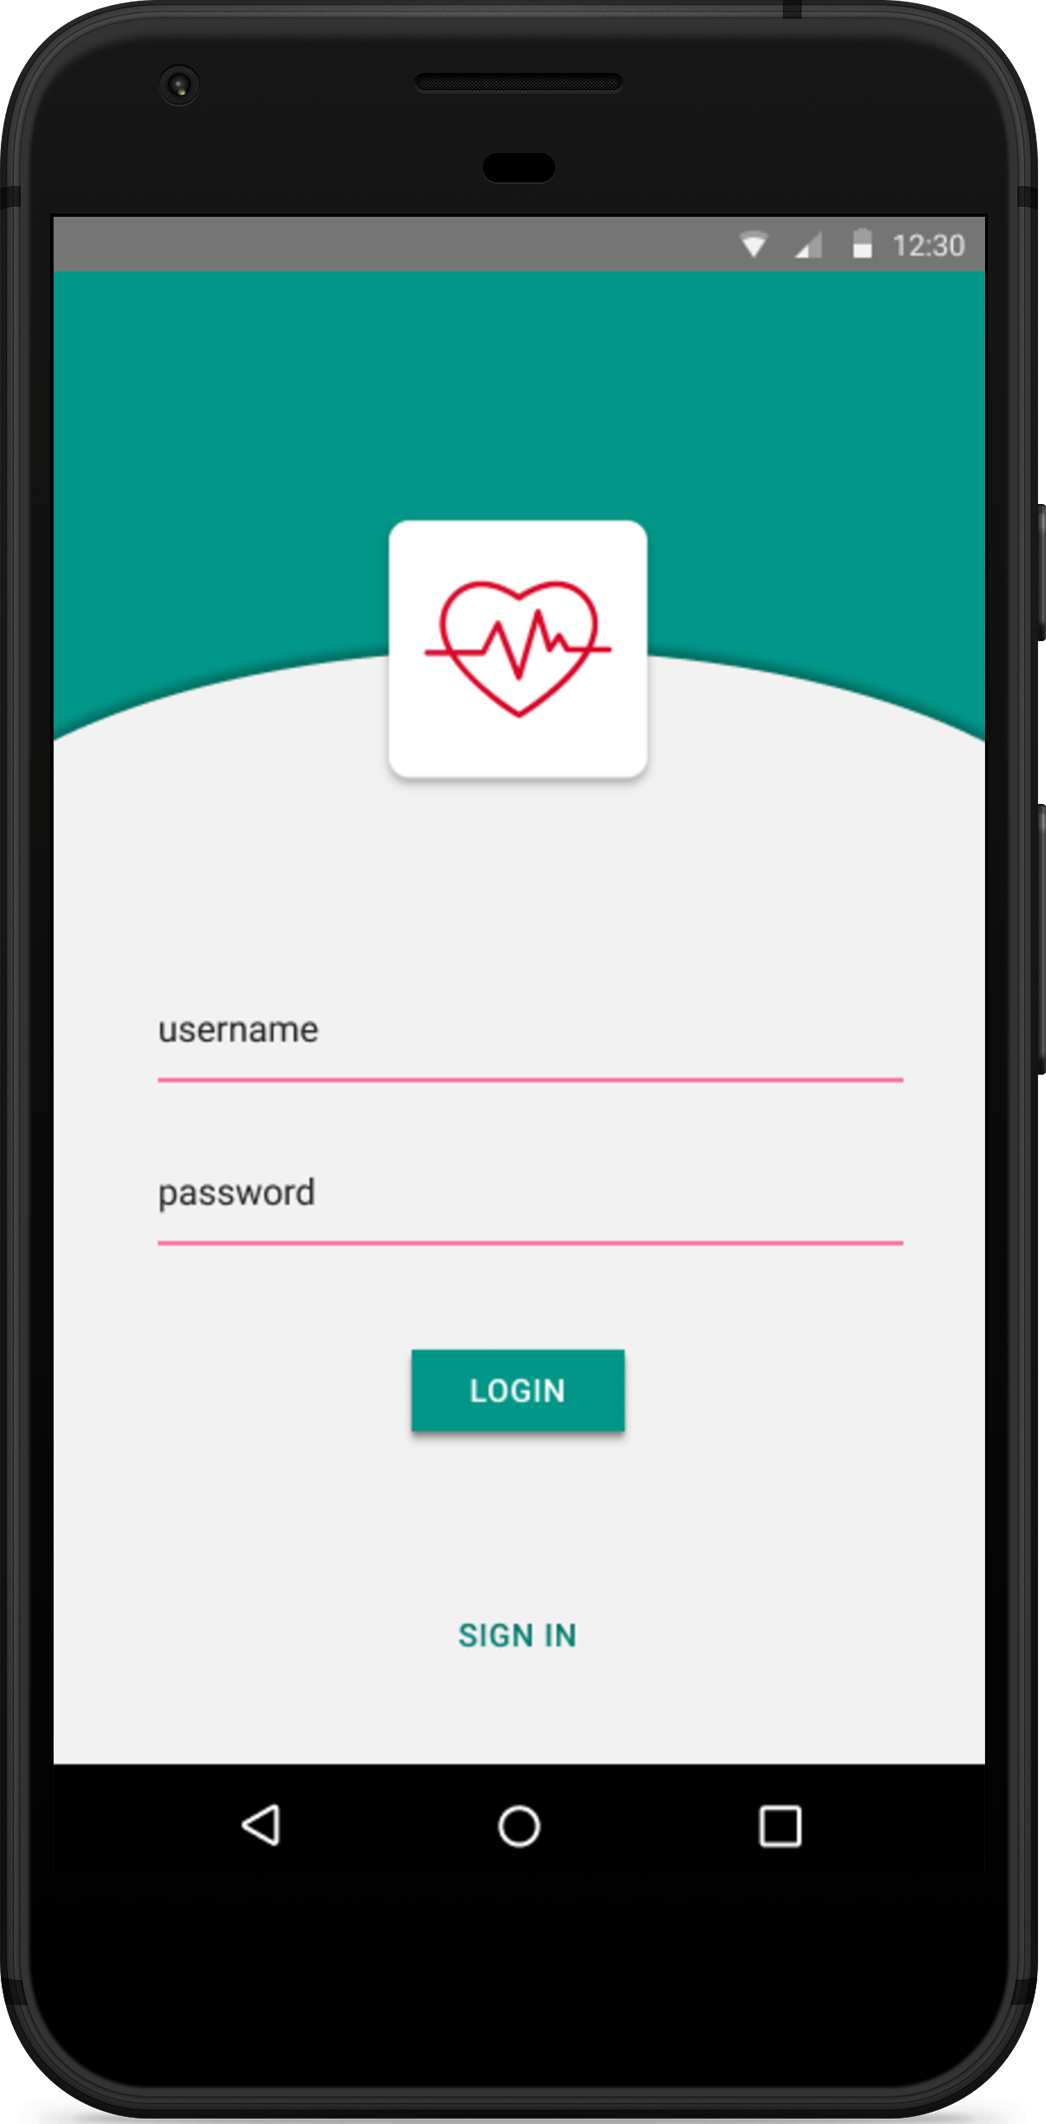
\includegraphics[width=\linewidth]{images/mockup/LoginPage.png}
		\caption{Login page}
		\label{mock_login}
	\end{subfigure}
	%
	\begin{subfigure}[b]{0.45\linewidth}
		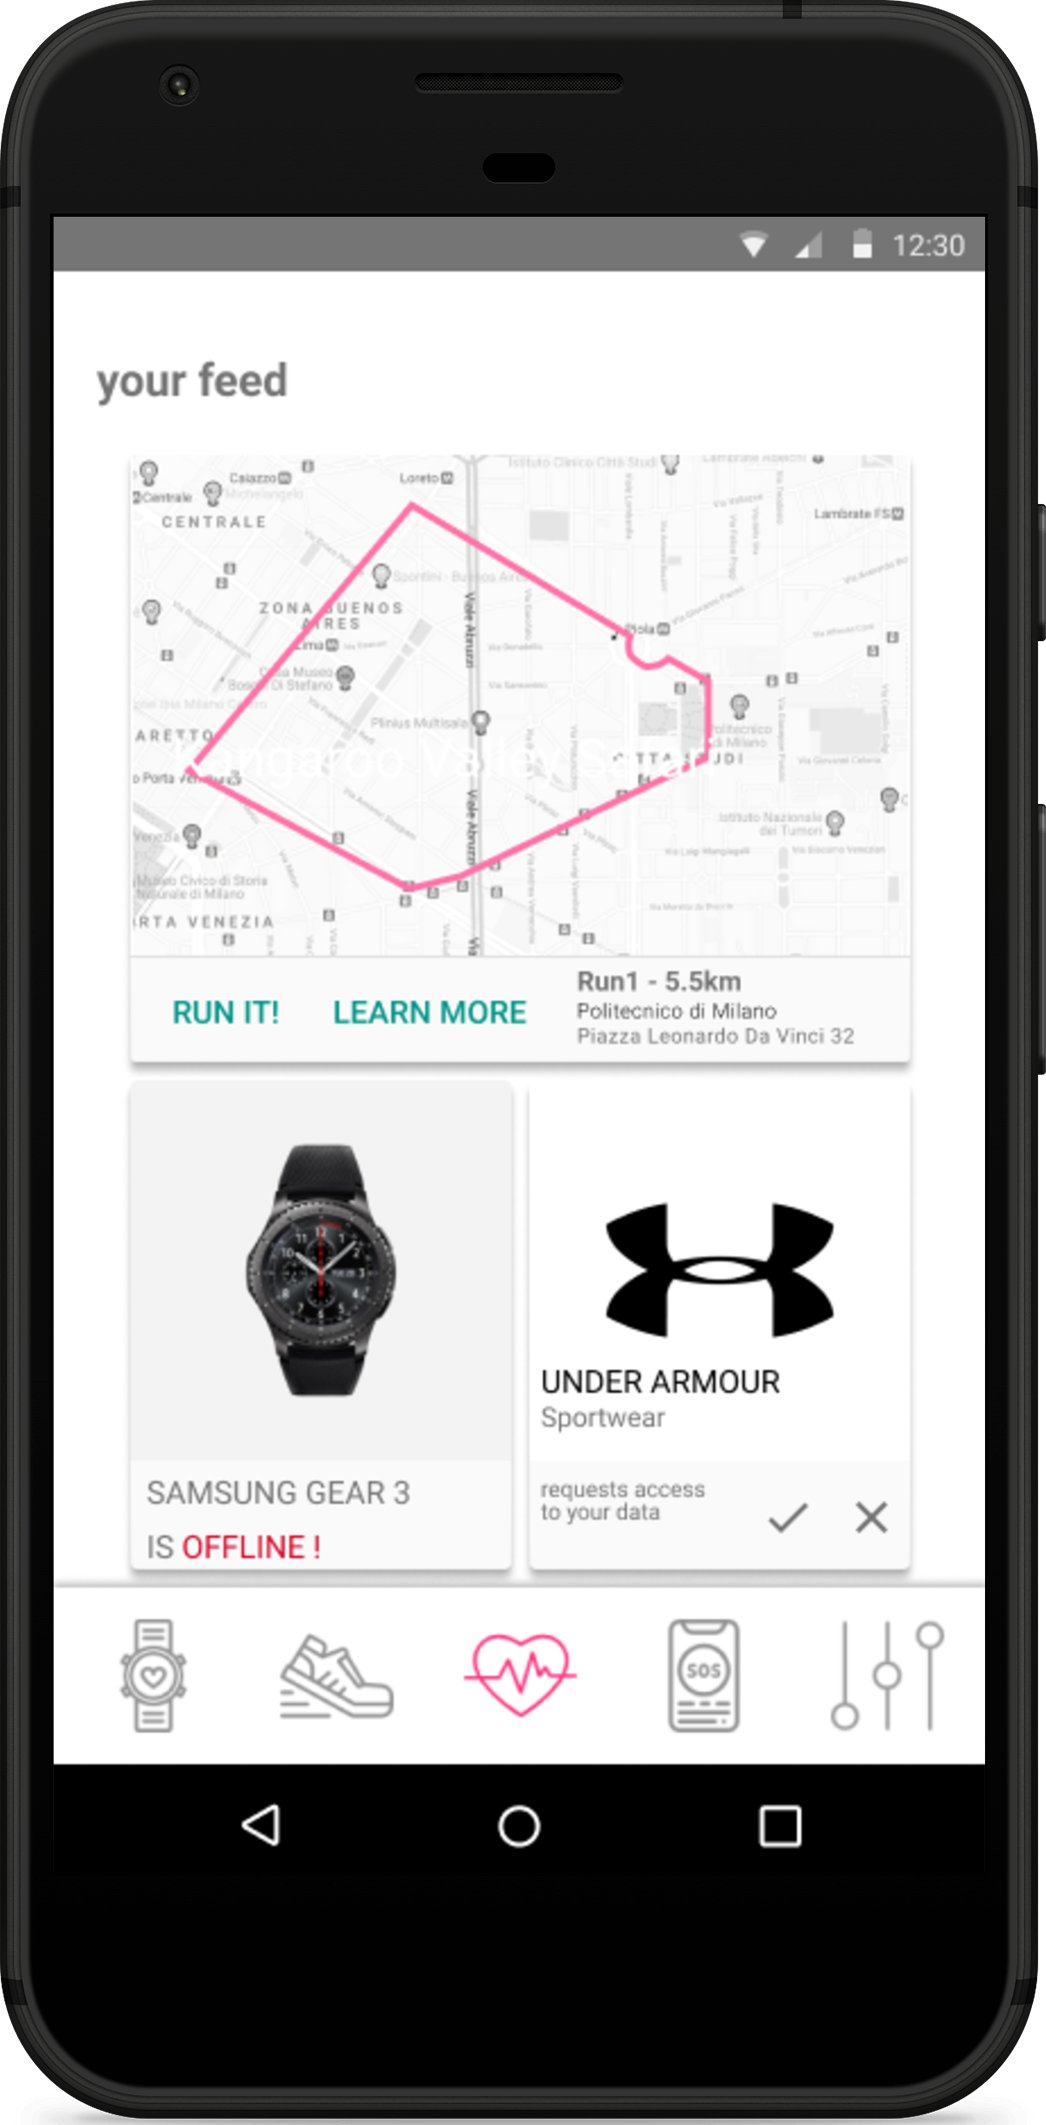
\includegraphics[width=\linewidth]{images/mockup/MainFeed.png}
		\caption{Main feed}
		\label{mock_mainfeed}
	\end{subfigure}
	\caption{}
\end{figure}

\begin{figure}[H]
	\centering
	\begin{subfigure}[b]{0.45\linewidth}
		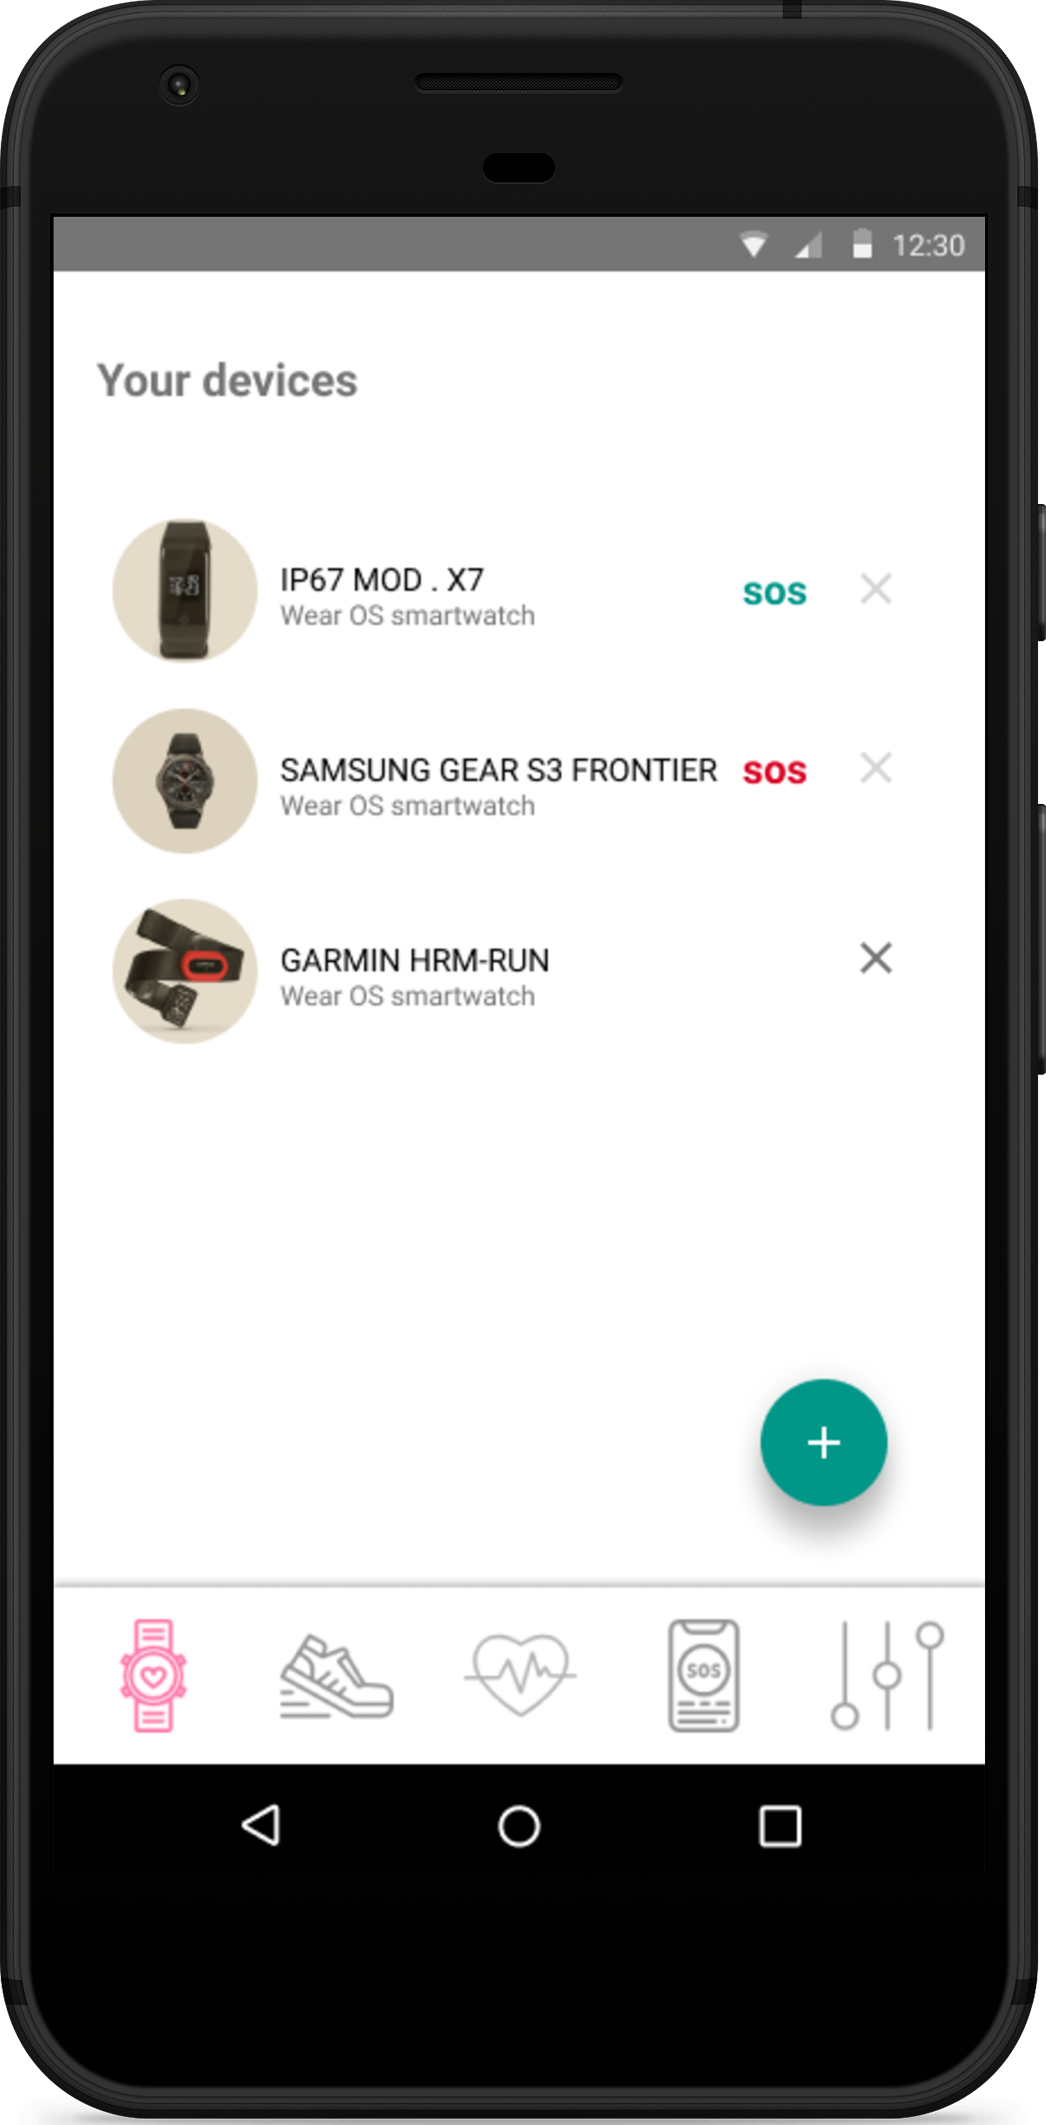
\includegraphics[width=\linewidth]{images/mockup/UserDevices.png}
		\caption{User's devices}
		\label{mock_userDevices}
	\end{subfigure}
	%
	\begin{subfigure}[b]{0.45\linewidth}
		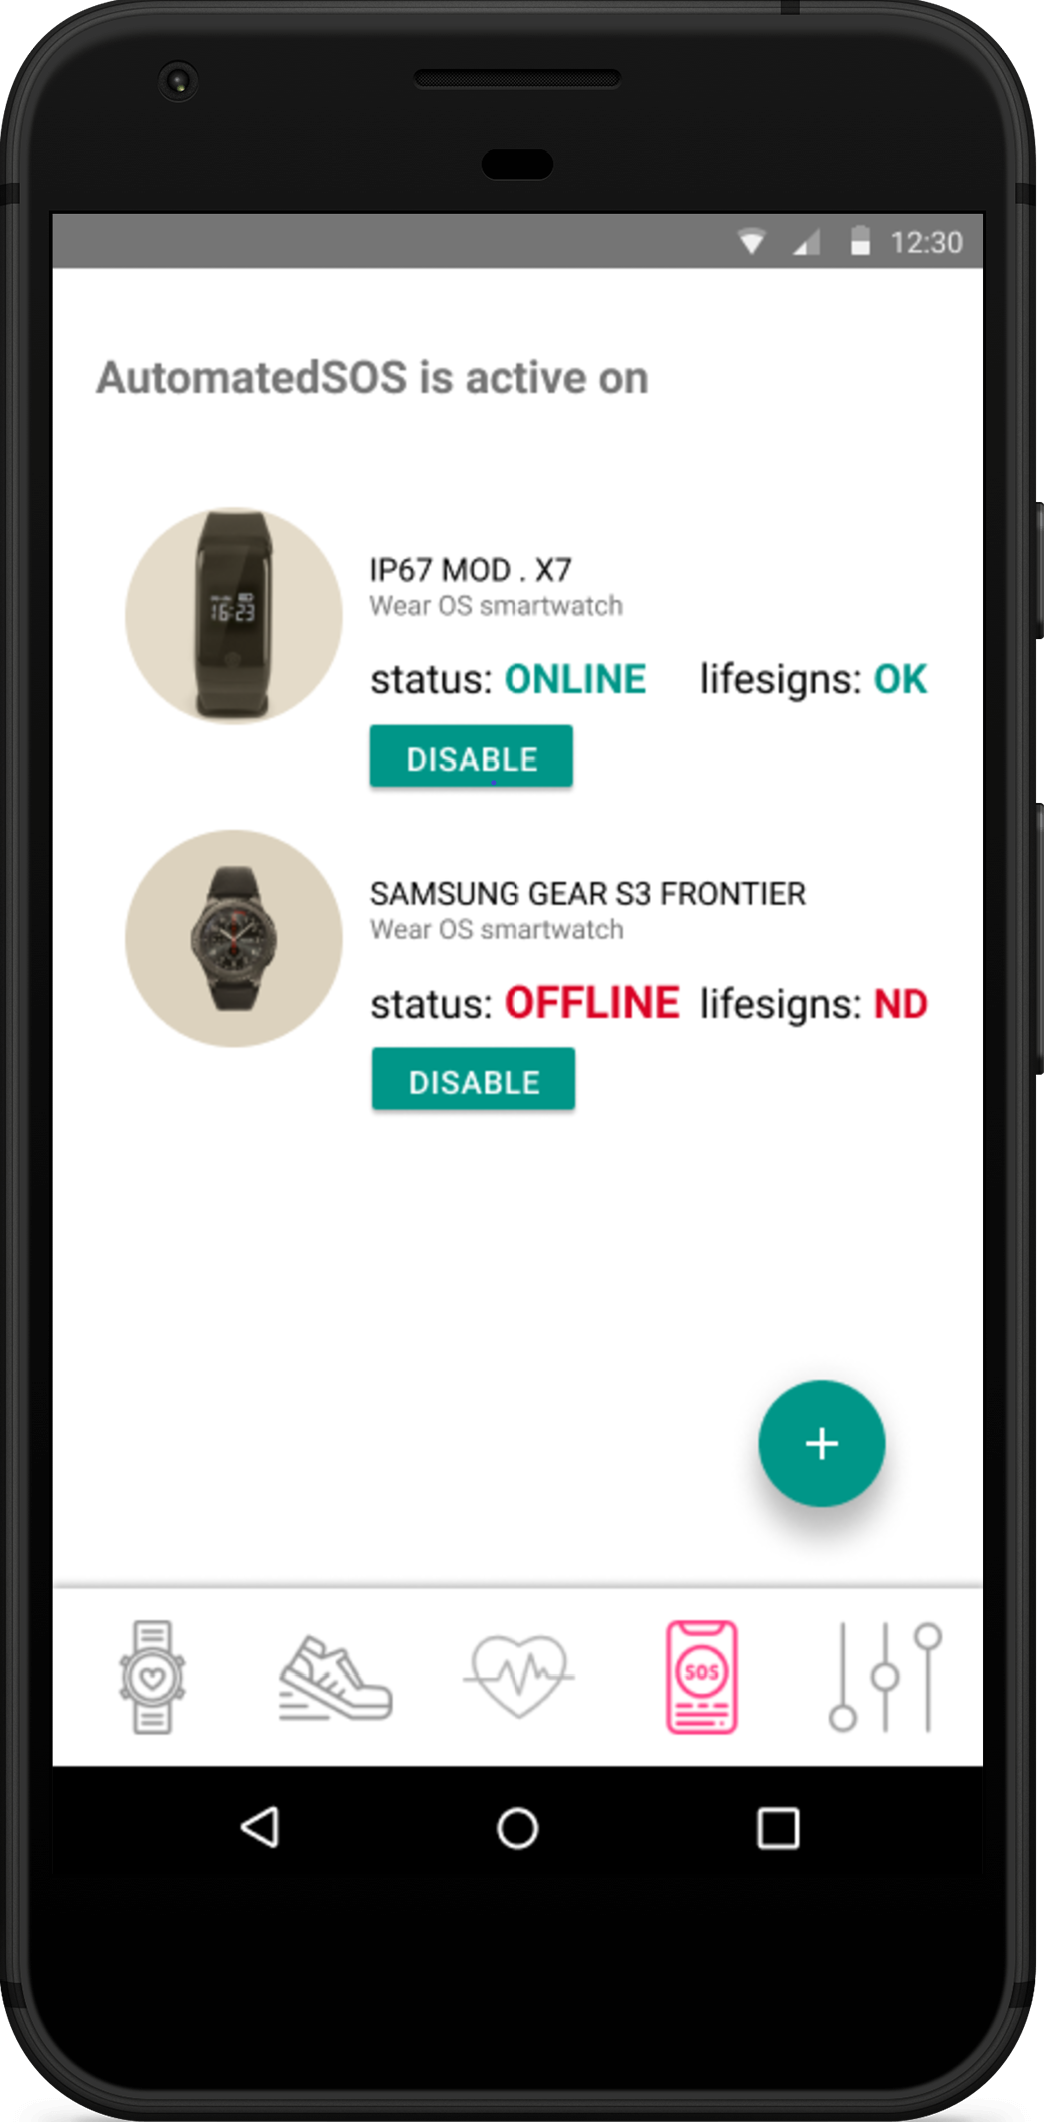
\includegraphics[width=\linewidth]{images/mockup/AutomatedSOS2.png}
		\caption{automatedSOS}
		\label{mock_automatedSOS}
	\end{subfigure}
	\caption{}
\end{figure}

\begin{figure}[H]
	\centering
	\begin{subfigure}[b]{0.45\linewidth}
		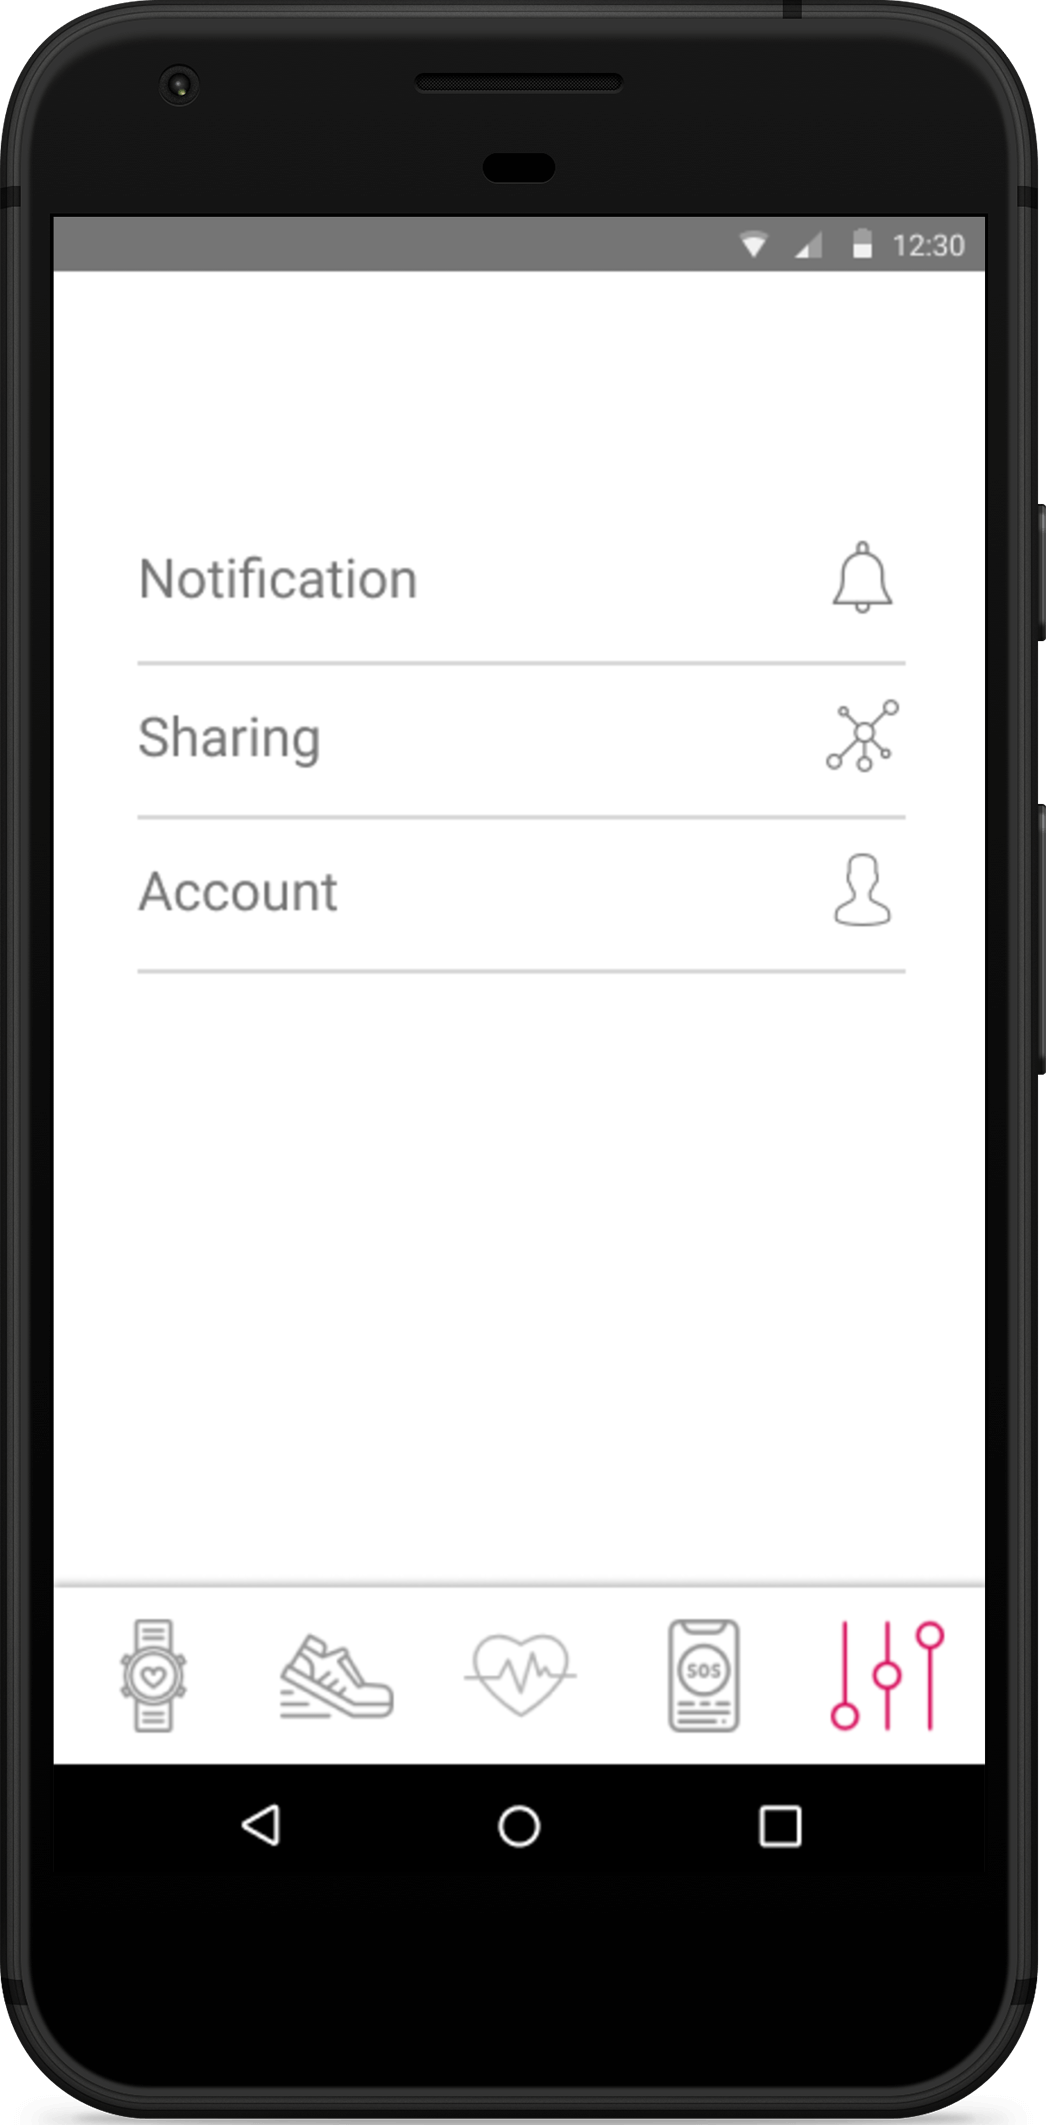
\includegraphics[width=\linewidth]{images/mockup/Settings.png}
		\caption{settings}
		\label{mock_settings}
	\end{subfigure}
	%
	\begin{subfigure}[b]{0.45\linewidth}
		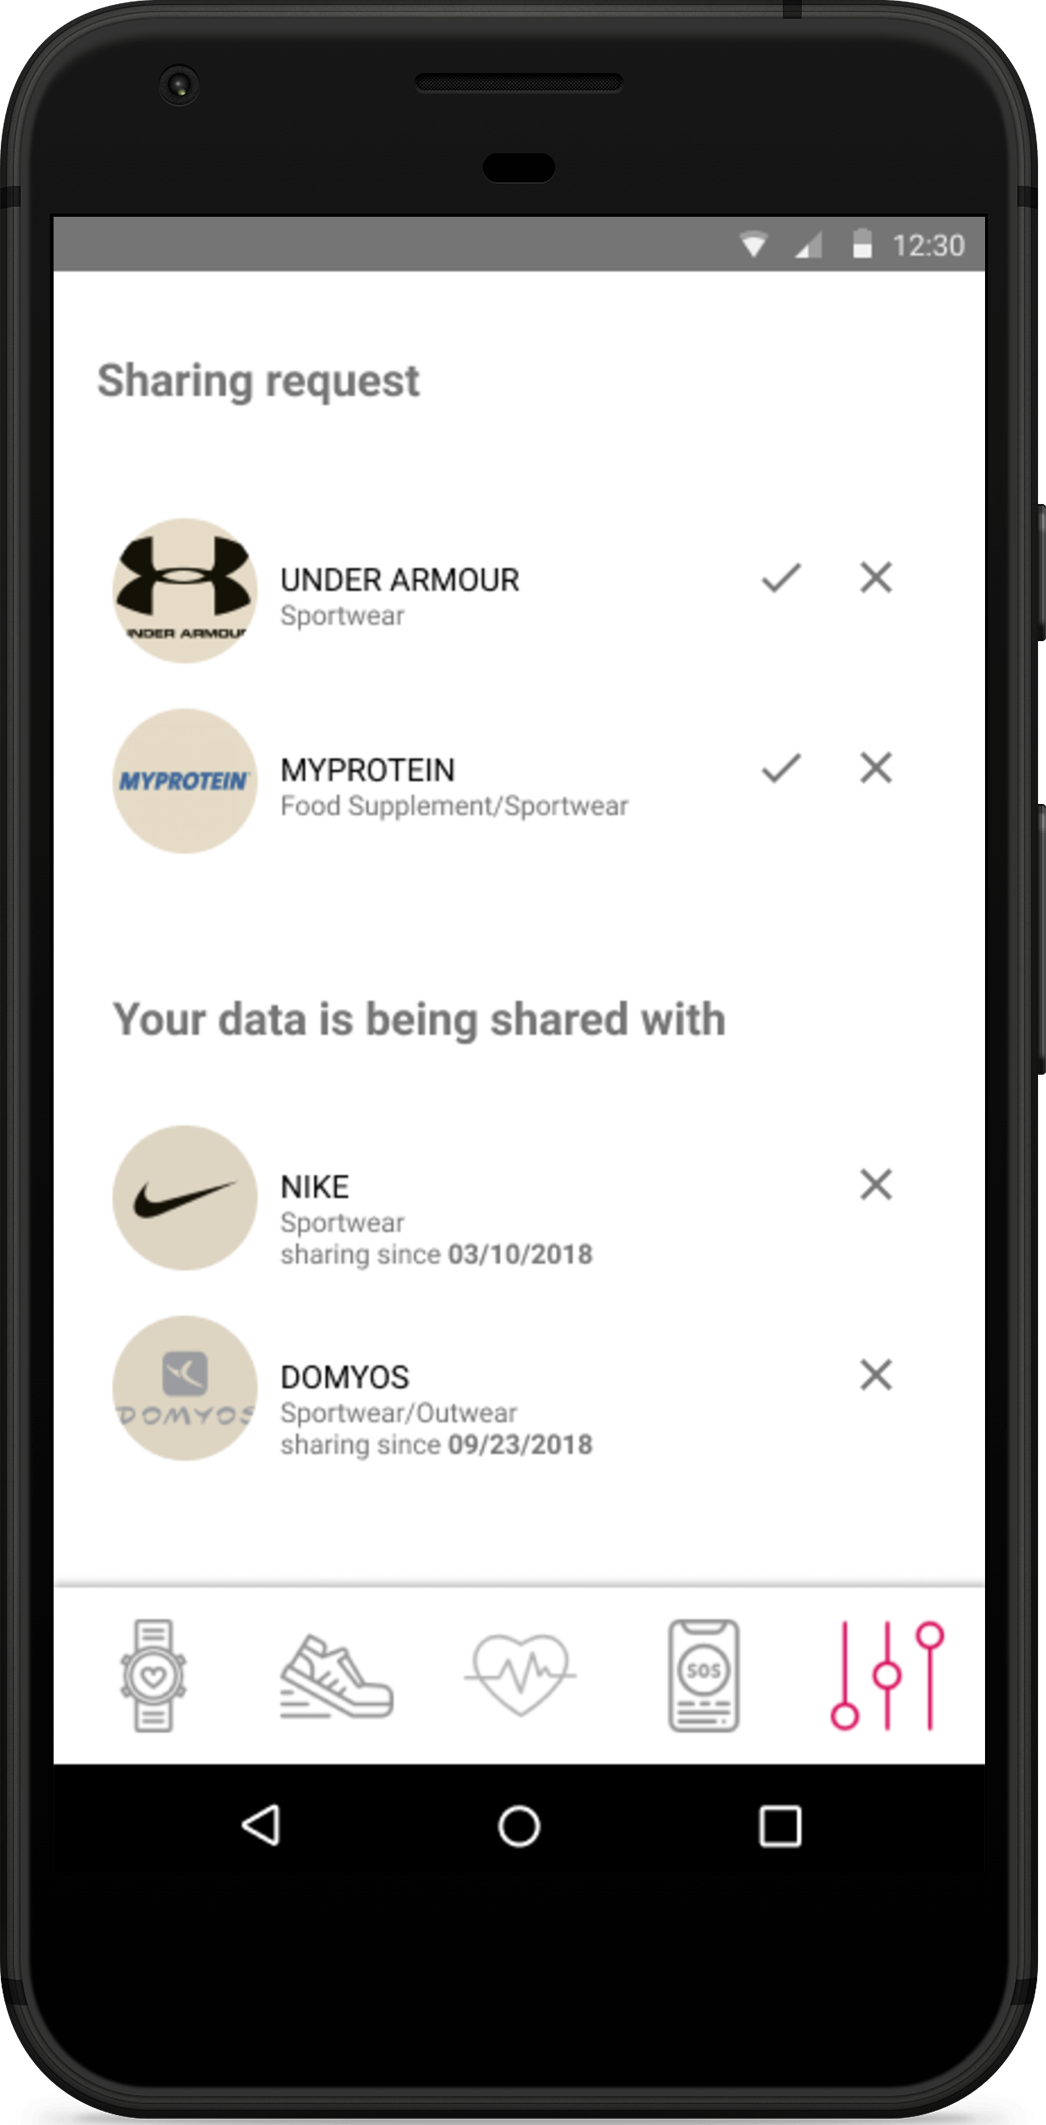
\includegraphics[width=\linewidth]{images/mockup/SharingCenter.png}
		\caption{sharing center}
		\label{mock_sharingCenter}
	\end{subfigure}
	\caption{}
\end{figure}

\begin{figure}[H]
	\centering
	\begin{subfigure}[b]{0.45\linewidth}
		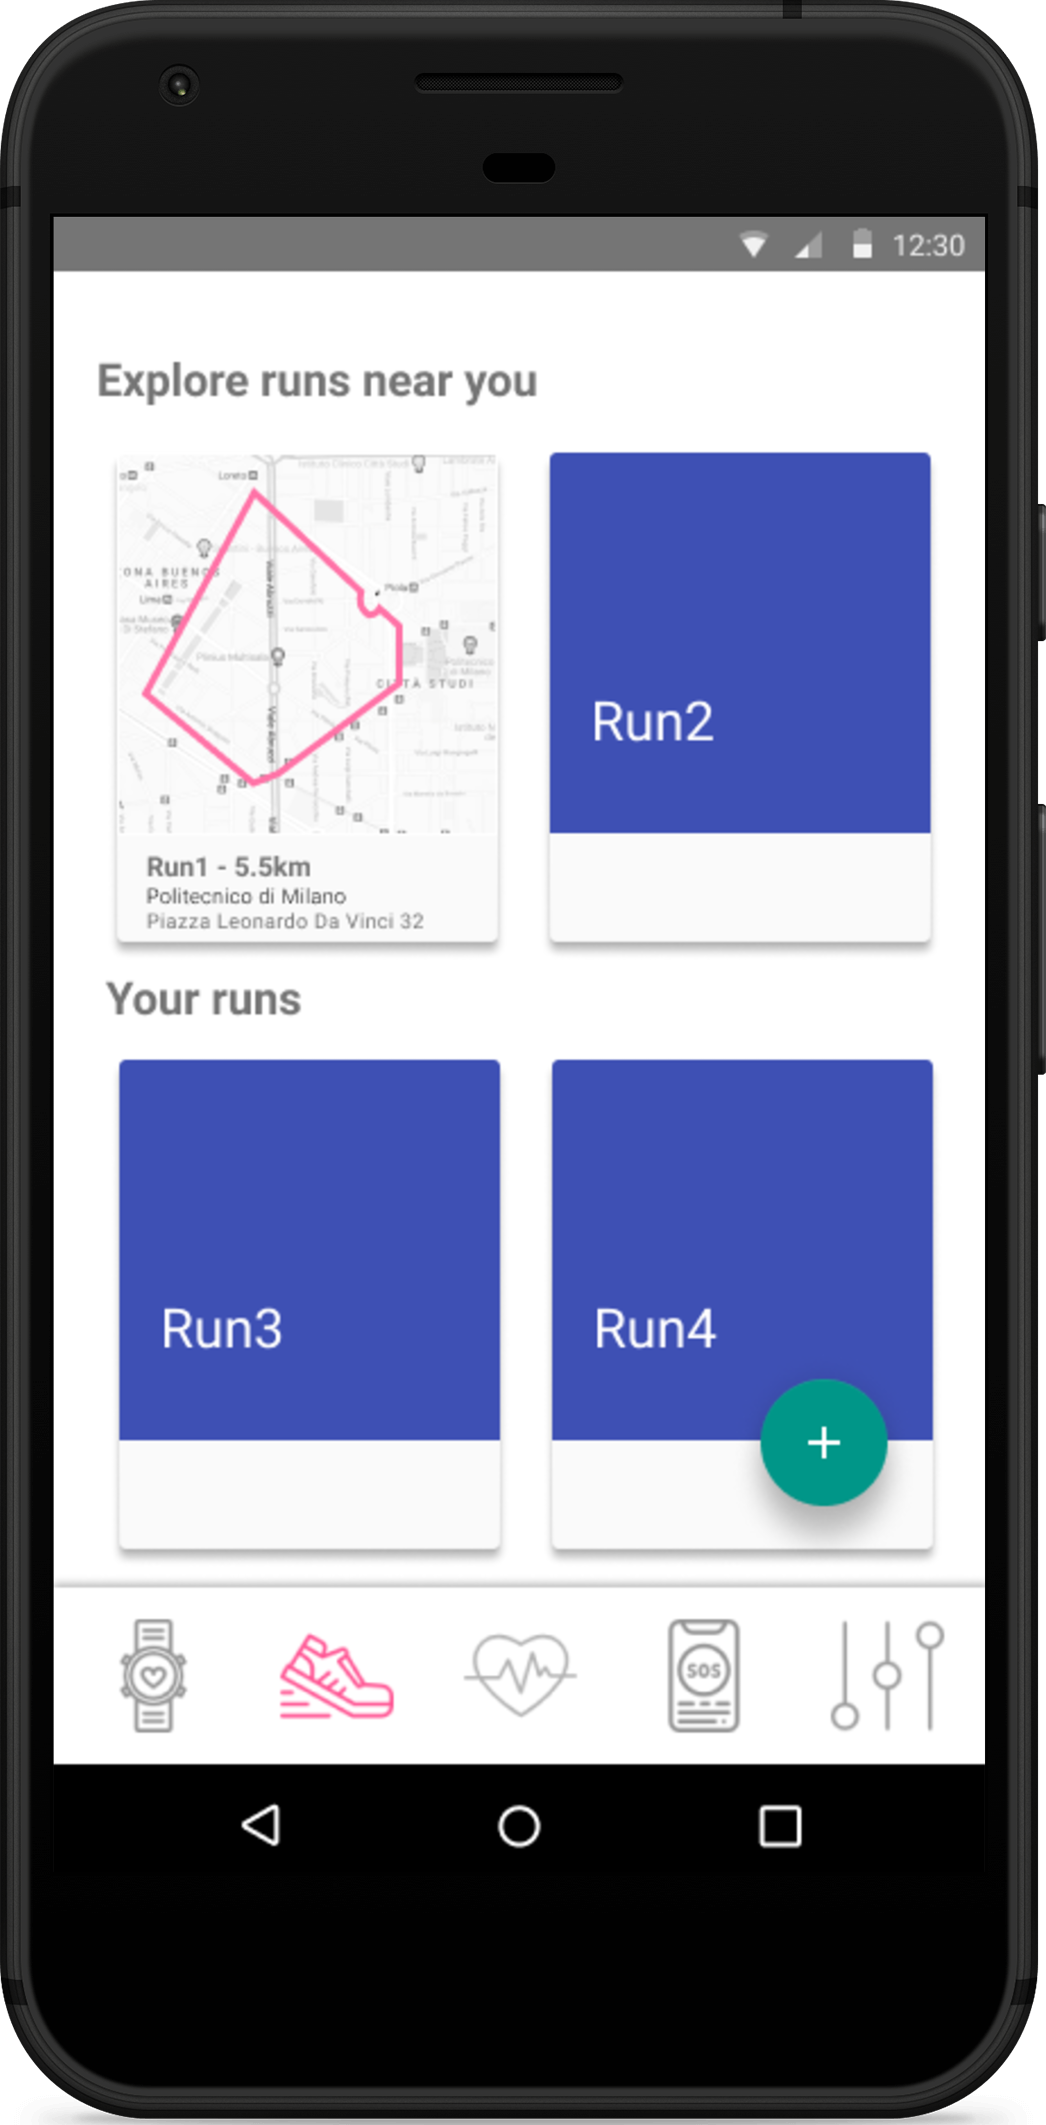
\includegraphics[width=\linewidth]{images/mockup/Track4Run.png}
		\caption{Running events}
		\label{mock_track4Run}
	\end{subfigure}
	%
	\begin{subfigure}[b]{0.45\linewidth}
		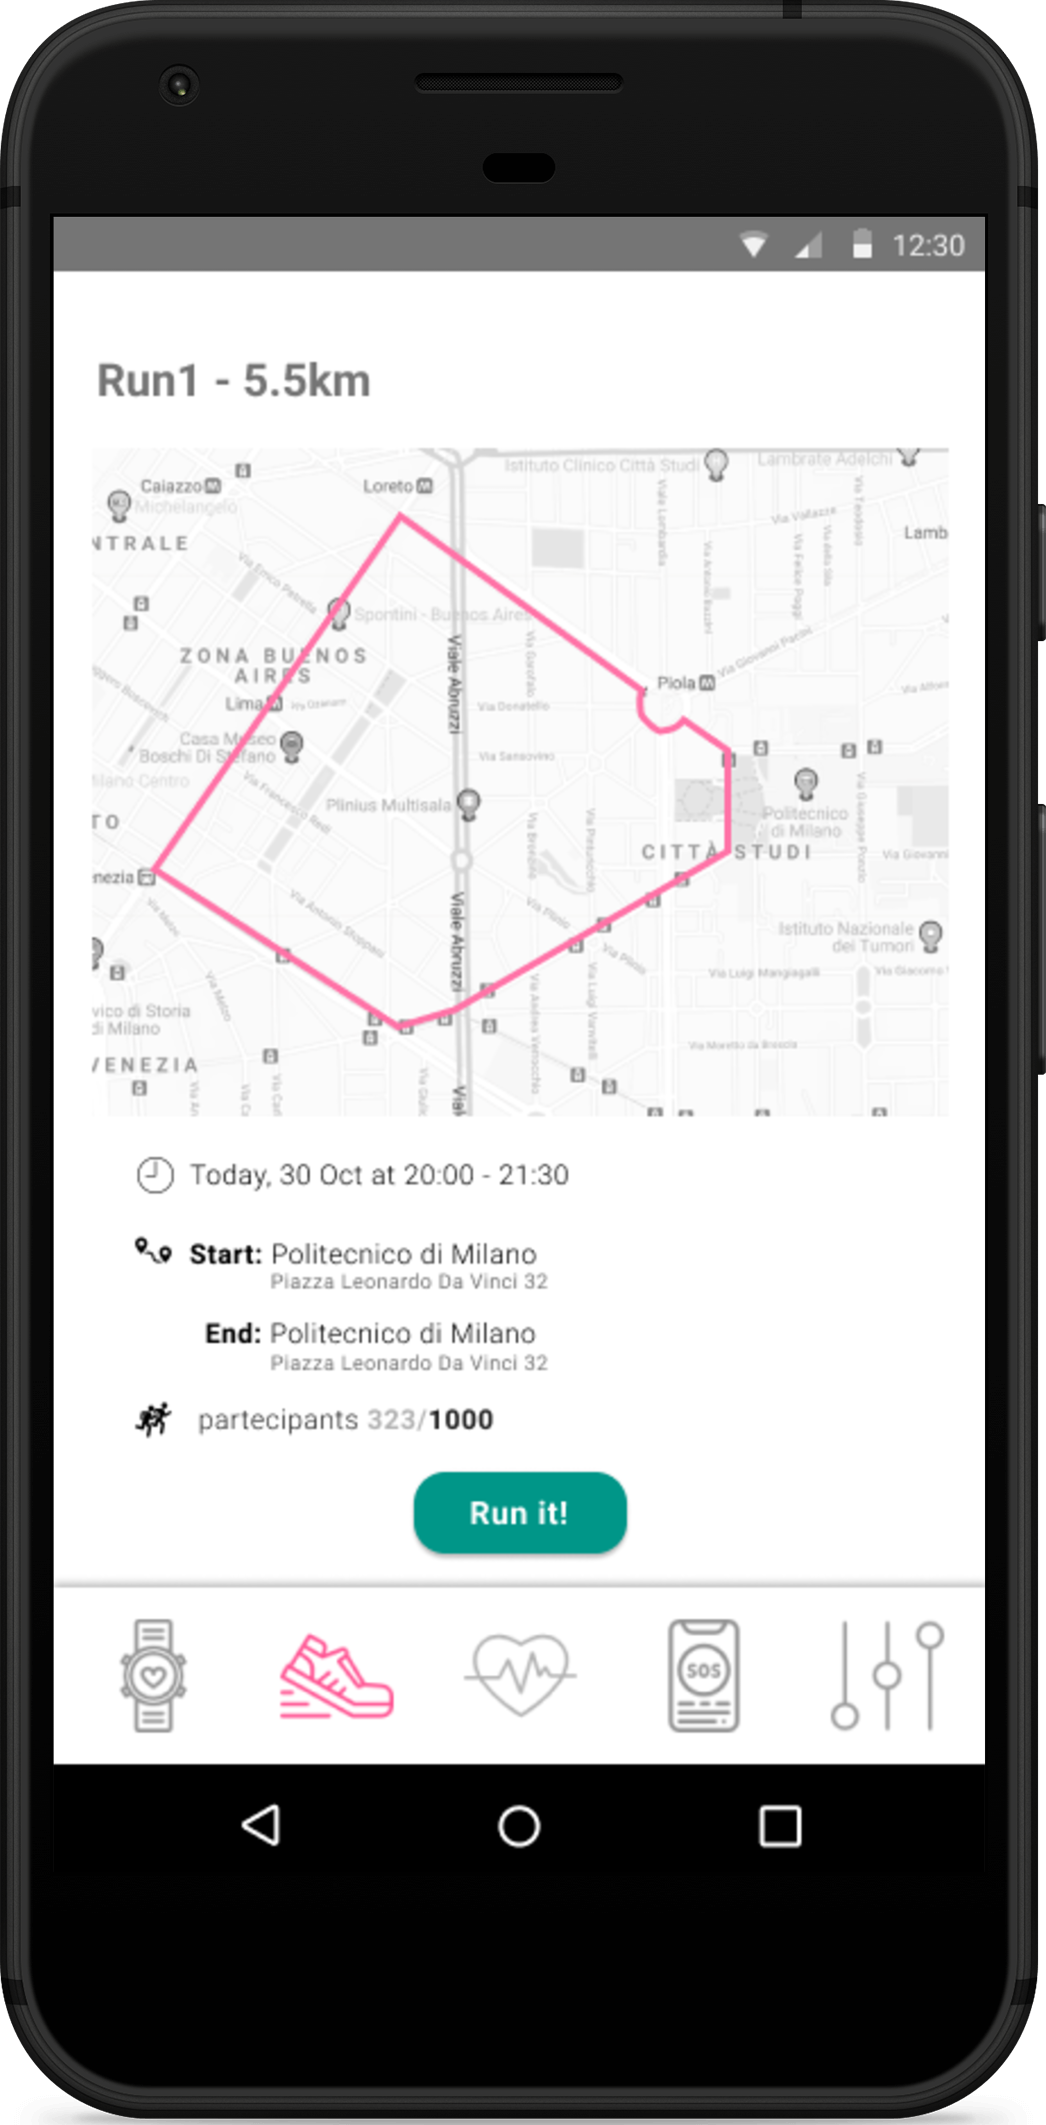
\includegraphics[width=\linewidth]{images/mockup/RunPage.png}
		\caption{Running event details}
		\label{mock_runPage}
	\end{subfigure}
	\caption{}
\end{figure}


\begin{figure}[H]
	\centering
	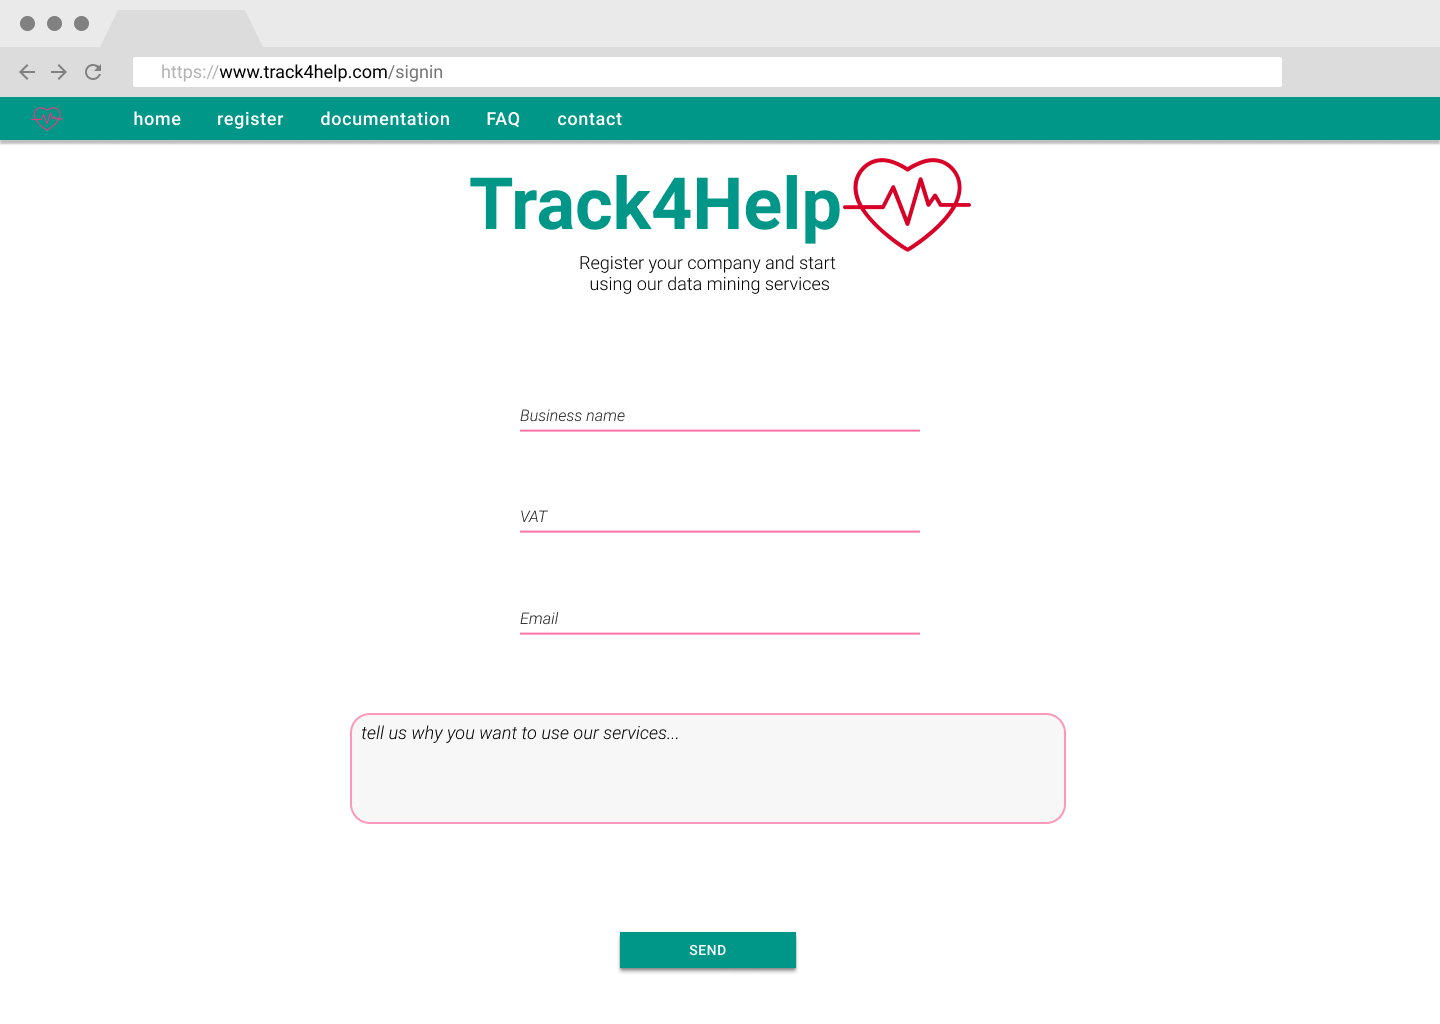
\includegraphics[scale=0.3]{images/mockup/webpage.png}
	\caption{sign in forms for Track4Help}
	\label{mockup_webpage}
\end{figure}
The website of Track4Help will offer a simple form to register a company and the API documentations for developers.

\subsubsection{Hardware requirements}

For using our services, the end customer will need a wearable device with appropriate sensors and interfaces (GPS, heart rate \& pressure, etc.) to capture the location and body parameters to our system. A smartphone will also be needed to be paired with such wearable device.

The third party company on the other hand won't need any particular interface, any device capable of communicating data through HTTPS protocol will be fine.

\subsubsection{Software interfaces}

The application makes use of the following externally developed services:

\begin{description}

	\item [Google Maps] For the Track4Run service, we use Google's maps service in order to let the spectators view the position of the runners; also, for a running event organizer, we give the possibility of defining and vieweing the path for the run on the interactive map.

	\item [Ambulance dispatching system] For the AutomatedSOS service, we use external software in order to be able to communicate with the ambulances and to track their position.

\end{description}


\subsubsection{Communication interfaces}

Communication between the customer's wearable device and his/her smartphone will take place through Bluetooth Low Energy protocol, and the one between such smartphone and our system through HTTPS, using a Wi-Fi or 3G/4G internet connection.

Communication between a third party company and our system will go through HTTPS procotol.


\subsection{Functional requirements}
	\subsubsection{Use Cases}
	\begin{figure}[H]
		\centering
		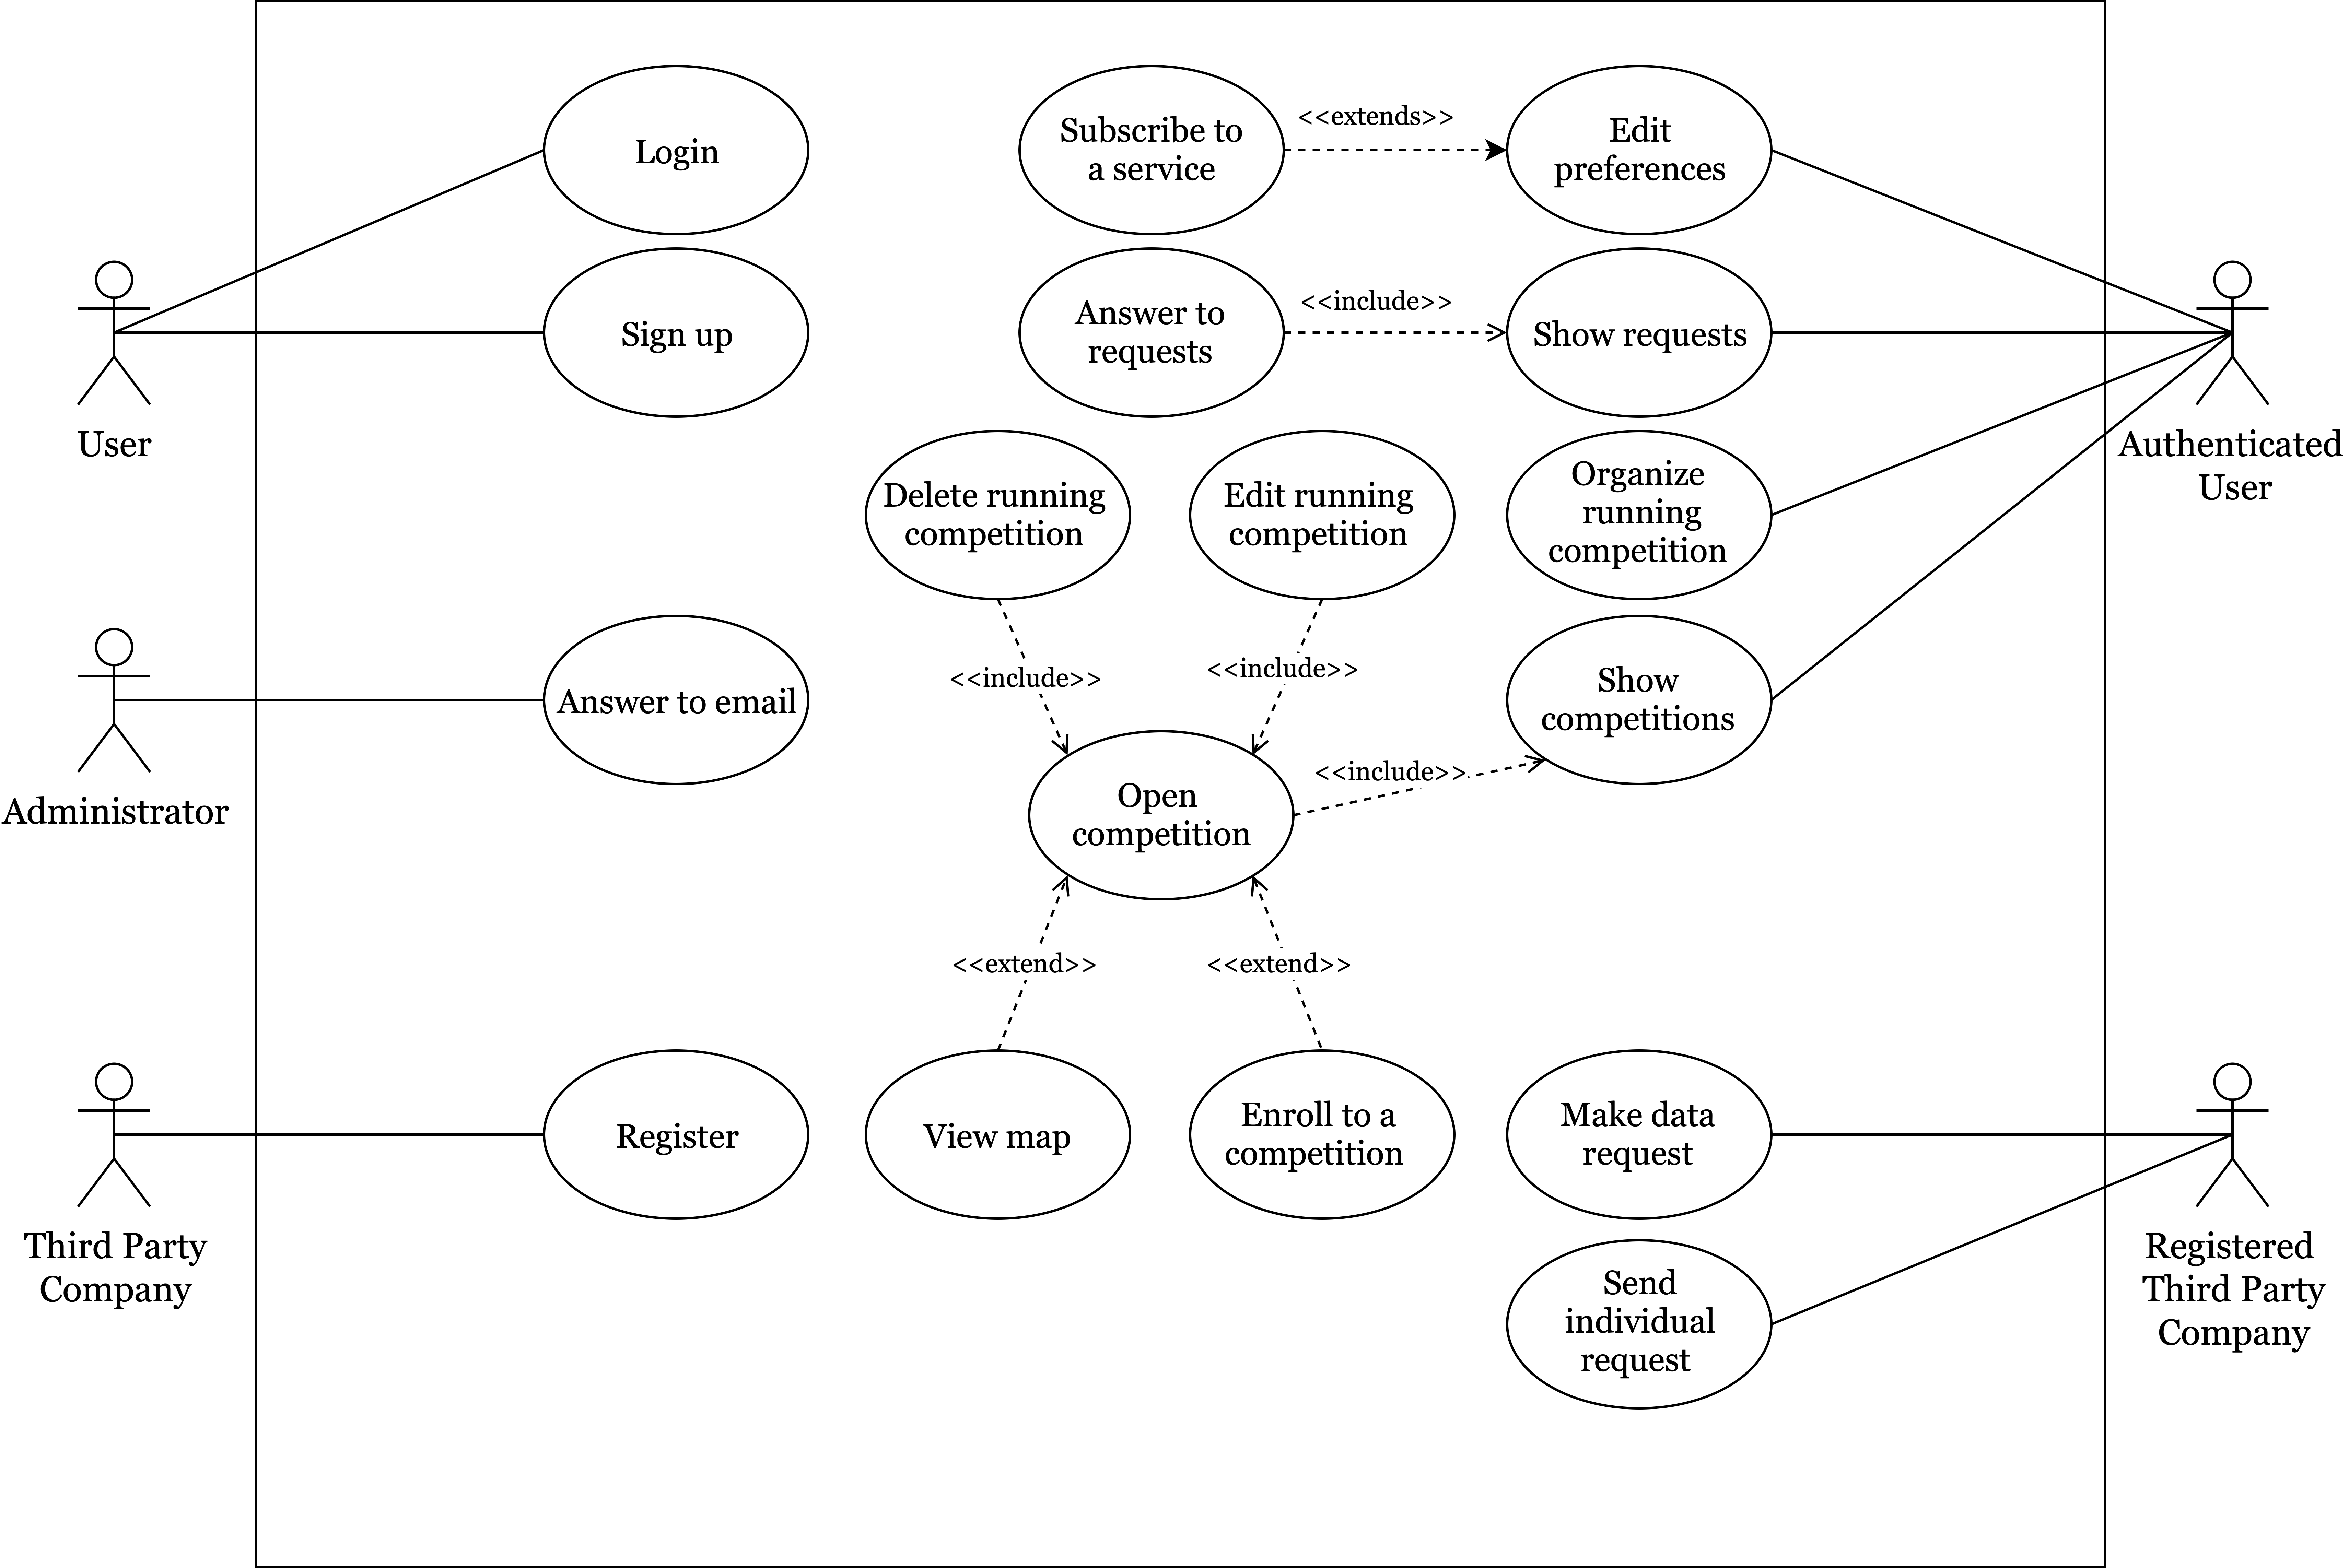
\includegraphics[scale=.052]{images/useCaseTrackMe.png}
		\caption{Use Case Diagram \label{fig:Use Case Diagram}}
	\end{figure}
	\begin{center}
		\begin{tabular}{p{3cm}p{8.28cm}}
			\hline
			\textbf{Use Case} & Sign up\\
			\hline
			\textbf{Actor} & User\\
			\hline
			\textbf{Entry condition} & The user has installed the application on his/her device.\\
			\hline
			\textbf{Flow of events} & \begin{enumerate}
				\linespread{0}\item The user clicks "Sign Up".
				\linespread{0}\item The user fills all mandatory fields.
				\linespread{0}\item The user accepts the privacy policies.
				\linespread{0}\item The user clicks "Confirm".
			\end{enumerate}\\
			\hline
			\textbf{Exit condition} & The user is registered and now he/she can log in to use the application.\\
			\hline
			\textbf{Exception} & \begin{enumerate}
				\linespread{0}\item The user is already registered.
				\linespread{0}\item The user doesn't fill all mandatory fields.
				\linespread{0}\item The user enters invalid data.
			\end{enumerate}\\
			\hline
			\textbf{Note} & When an exception occurs the user is notified and the application return to previous page.\\
			\hline
		\end{tabular}
	\end{center}
	\vspace*{3cm}
	\begin{center}
		\begin{tabular}{p{3cm}p{8.28cm}}
			\hline
			\textbf{Use Case} & Login\\
			\hline
			\textbf{Actor} & User\\
			\hline
			\textbf{Entry condition} & The user has installed the application and it is open on his/her device.\\
			\hline
			\textbf{Flow of events} & \begin{enumerate}
				\linespread{0}\item The user clicks "Log In".
				\linespread{0}\item The user enters username and password.
				\linespread{0}\item The user decides if he/she wants to be remembered by the system clicking on the relative checkbox.
				\linespread{0}\item The user clicks "Confirm".
				\linespread{0}\item If the user chose to be remembered, next time the use case ends without asking username and password.
			\end{enumerate}\\
			\hline
			\textbf{Exit condition} & The user is on the home page of the application.\\
			\hline
			\textbf{Exception} & \begin{enumerate}
				\linespread{0}\item The user enters invalid data.
				\linespread{0}\item The user doesn't fill all fields.
			\end{enumerate}\\
			\hline
			\textbf{Note} & When an exception occurs the user is notified and the application return to previous page.\\
			\hline
		\end{tabular}
	\end{center}
	\vspace*{3cm}
	\begin{center}
		\begin{tabular}{p{3cm}p{8.28cm}}
			\hline
			\textbf{Use Case} & Register\\
			\hline
			\textbf{Actor} & Third Party Company\\
			\hline
			\textbf{Entry condition} & The third party company is on TrackMe website.\\
			\hline
			\textbf{Flow of events} & \begin{enumerate}
				\linespread{0}\item The third party company goes to the registering page.
				\linespread{0}\item The third party company fills all mandatory fields.
				\linespread{0}\item The third party company clicks on "Send" button. An email with the informations is sent to TrackMe.
			\end{enumerate}\\
			\hline
			\textbf{Exit condition} & The third party company is waiting for the Data4Help API key to be received.\\
			\hline
			\textbf{Exception} & \begin{enumerate}
				\linespread{0}\item The third party company enters invalid data.
				\linespread{0}\item The third party company doesn't fill all fields.
				\linespread{0}\item Sending the email fails.
			\end{enumerate}\\
			\hline
			\textbf{Note} & When an exception occurs the email is not sent and the third party company is notified.\\
			\hline
		\end{tabular}
	\end{center}
	\vspace*{3cm}
	\begin{center}
		\begin{tabular}{p{3cm}p{8.28cm}}
			\hline
			\textbf{Use Case} & Answer to email\\
			\hline
			\textbf{Actor} & Administrator\\
			\hline
			\textbf{Entry condition} & The administrator has received an email from a third party company.\\
			\hline
			\textbf{Flow of events} & \begin{enumerate}
				\linespread{0}\item The administrator reads the email.
				\linespread{0}\item If the third party company is legit the administrator sends the API key.
				\linespread{0}\item If the third party company isn't legit the administrator sends a rejection email.
			\end{enumerate}\\
			\hline
			\textbf{Exit condition} & The third party company receives the API key.\\
			\hline
			\textbf{Exception} & \begin{enumerate}
				\linespread{0}\item Sending the email fails.
			\end{enumerate}\\
			\hline
			\textbf{Note} & When sending the email fails the administrator is notified.\\
			\hline
		\end{tabular}
	\end{center}
	\vspace*{3cm}
	\begin{center}
		\begin{tabular}{p{3cm}p{8.28cm}}
			\hline
			\textbf{Use Case} & Edit prefernces\\
			\hline
			\textbf{Actor} & Authenticated User\\
			\hline
			\textbf{Entry condition} & The authenticated user is on the home page of the application.\\
			\hline
			\textbf{Flow of events} & \begin{enumerate}
				\linespread{0}\item The authenticated user selects what service he/she wants to activate: AutomatedSOS, Track4Run.
				\linespread{0}\item The authenticated user can delete the authorizations to give data to the third party companies.
				\linespread{0}\item The authenticated user can edit personal informations.
			\end{enumerate}\\
			\hline
			\textbf{Exit condition} & The preferences is saved.\\
			\hline
			\textbf{Exception}\\
			\hline
		\end{tabular}
	\end{center}
	\vspace*{3cm}
	\begin{center}
		\begin{tabular}{p{3cm}p{8.28cm}}
			\hline
			\textbf{Use Case} & Subscribe to a service.\\
			\hline
			\textbf{Actor} & Authenticated User\\
			\hline
			\textbf{Entry condition} & The authenticated user wants to subscribe or unsubscribe to AutomatedSOS and Track4Run.\\
			\hline
			\textbf{Flow of events} & \begin{enumerate}
				\linespread{0}\item The authenticated user opens the preferences.
				\linespread{0}\item The authenticated user clicks a box to subscribe himself to a service.
				\linespread{0}\item If it's required, the authenticated user connects his/her wearable device.
			\end{enumerate}\\
			\hline
			\textbf{Exit condition} & The authenticated user is subriscribed to the desired services.\\
			\hline
			\textbf{Exception} & \begin{enumerate}
				\linespread{0}\item The authenticated user doesn't connect the wearable device when requested.
			\end{enumerate}\\
			\hline
			\textbf{Note} & When an exception occurs the preferences are not saved.\\
			\hline
		\end{tabular}
	\end{center}
	\vspace*{3cm}
	\begin{center}
		\begin{tabular}{p{3cm}p{8.28cm}}
			\hline
			\textbf{Use Case} & Show requests\\
			\hline
			\textbf{Actor} & Authenticated User\\
			\hline
			\textbf{Entry condition} & The authenticated user is on the home page and wants to see the requests.\\
			\hline
			\textbf{Flow of events} & \begin{enumerate}
				\linespread{0}\item The authenticated user opens the requests page.
			\end{enumerate}\\
			\hline
			\textbf{Exit condition} & The requests page is opened and all the requets are visible.\\
			\hline
			\textbf{Exception}\\
			\hline
		\end{tabular}
	\end{center}
	\vspace*{3cm}
	\begin{center}
		\begin{tabular}{p{3cm}p{8.28cm}}
			\hline
			\textbf{Use Case} & Answer to requests\\
			\hline
			\textbf{Actor} & Authenticated User\\
			\hline
			\textbf{Entry condition} & The authenticated user is on the requests page.\\
			\hline
			\textbf{Flow of events} & \begin{enumerate}
				\linespread{0}\item The authenticated user opens a request.
				\linespread{0}\item The authenticated user clicks on "Accept" or "Refuse".
				\linespread{0}\item When the user approves a data request of a third party company all user's data becomes available to it.
			\end{enumerate}\\
			\hline
			\textbf{Exit condition} & The answers are saved. The approved requests make the relative third party company able to access currently stored data and to subscribe to new collected data.\\
			\hline
			\textbf{Exception}\\
			\hline
		\end{tabular}
	\end{center}
	\vspace*{3cm}
	\begin{center}
		\begin{tabular}{p{3cm}p{8.28cm}}
			\hline
			\textbf{Use Case} & Organize running event\\
			\hline
			\textbf{Actor} & Authenticated User\\
			\hline
			\textbf{Entry condition} & The authenticated user is on the home page and wants to organize a running event.\\
			\hline
			\textbf{Flow of events} & \begin{enumerate}
				\linespread{0}\item The authenticated user clicks "New running event".
				\linespread{0}\item The authenticated user selects the route, date and time.
				\linespread{0}\item The authenticated user clicks "Confirm".
			\end{enumerate}\\
			\hline
			\textbf{Exit condition} & The running event is organized and now users can view it and enroll to it.\\
			\hline
			\textbf{Exception} & \begin{enumerate}
				\linespread{0}\item There is another running event in the same place, date and time.
				\linespread{0}\item The route, date or time selected are not valid.
			\end{enumerate}\\
			\hline
			\textbf{Note} & When an exception occurs the running event is not saved and the user is notified.\\
			\hline
		\end{tabular}
	\end{center}
	\vspace*{3cm}
	\begin{center}
		\begin{tabular}{p{3cm}p{8.28cm}}
			\hline
			\textbf{Use Case} & Show running events\\
			\hline
			\textbf{Actor} & Authenticated User\\
			\hline
			\textbf{Entry condition} & The authenticated user is on the home page and wants to view the running events.\\
			\hline
			\textbf{Flow of events} & \begin{enumerate}
				\linespread{0}\item The authenticated user clicks "Show running events".
			\end{enumerate}\\
			\hline
			\textbf{Exit condition} & All running events are visible to the user.\\
			\hline
			\textbf{Exception}\\
			\hline
		\end{tabular}
	\end{center}
	\vspace*{3cm}
	\begin{center}
		\begin{tabular}{p{3cm}p{8.28cm}}
			\hline
			\textbf{Use Case} & Open running event\\
			\hline
			\textbf{Actor} & Authenticated User\\
			\hline
			\textbf{Entry condition} & The authenticated user is on the running events page.\\
			\hline
			\textbf{Flow of events} & \begin{enumerate}
				\linespread{0}\item The authenticated user select a running event.
				\linespread{0}\item The authenticated user views all details of the running event.
			\end{enumerate}\\
			\hline
			\textbf{Exit condition} & The running event page is shown to the user.\\
			\hline
			\textbf{Exception}\\
			\hline
		\end{tabular}
	\end{center}
	\vspace*{3cm}
	\begin{center}
		\begin{tabular}{p{3cm}p{8.28cm}}
			\hline
			\textbf{Use Case} & Edit running event\\
			\hline
			\textbf{Actor} & Authenticated User\\
			\hline
			\textbf{Entry condition} & The authenticated user is the creator of the running event and he/she is on the running event page.\\
			\hline
			\textbf{Flow of events} & \begin{enumerate}
				\linespread{0}\item The authenticated user clicks on "Edit".
				\linespread{0}\item The authenticated user changes route, date and time.
				\linespread{0}\item The authenticated user clicks "Save".
			\end{enumerate}\\
			\hline
			\textbf{Exit condition} & The changes are saved\\
			\hline
			\textbf{Exception}& \begin{enumerate}
				\linespread{0}\item There is another running event in the same place, date and time.
				\linespread{0}\item The route, date or time selected are not valid.
			\end{enumerate}\\
			\hline
			\textbf{Note} & When an exception occurs the changes are not saved and the user is notified.\\
			\hline
		\end{tabular}
	\end{center}
	\vspace*{3cm}
	\begin{center}
		\begin{tabular}{p{3cm}p{8.28cm}}
			\hline
			\textbf{Use Case} & Delete running event\\
			\hline
			\textbf{Actor} & Authenticated User\\
			\hline
			\textbf{Entry condition} & The authenticated user is the creator of the running event and he/she is on the running event page.\\
			\hline
			\textbf{Flow of events} & \begin{enumerate}
				\linespread{0}\item The authenticated user clicks on "Delete".
			\end{enumerate}\\
			\hline
			\textbf{Exit condition} & The running event is deleted.\\
			\hline
			\textbf{Exception}& \begin{enumerate}
				\linespread{0}\item The user tries to delete a running event that is in progress.
			\end{enumerate}\\
			\hline
			\textbf{Note} & When an exception occurs the running event is not deleted and the user is notified.\\
			\hline
		\end{tabular}
	\end{center}
	\vspace*{3cm}
	\begin{center}
		\begin{tabular}{p{3cm}p{8.28cm}}
			\hline
			\textbf{Use Case} & Enroll in a running event\\
			\hline
			\textbf{Actor} & Authenticated User\\
			\hline
			\textbf{Entry condition} & The authenticated user is on the specific running event page and he/she isn't the creator of it.\\
			\hline
			\textbf{Flow of events} & \begin{enumerate}
				\linespread{0}\item The authenticated user clicks on "Enroll".
			\end{enumerate}\\
			\hline
			\textbf{Exit condition} & The user is enrolled to the running event selected.\\
			\hline
			\textbf{Exception}\\
			\hline
		\end{tabular}
	\end{center}
	\vspace*{3cm}
	\begin{center}
		\begin{tabular}{p{3cm}p{8.28cm}}
			\hline
			\textbf{Use Case} & View map\\
			\hline
			\textbf{Actor} & Authenticated User\\
			\hline
			\textbf{Entry condition} & The authenticated user is on the specific event page.\\
			\hline
			\textbf{Flow of events} & \begin{enumerate}
				\linespread{0}\item The authenticated user clicks on "Map".
			\end{enumerate}\\
			\hline
			\textbf{Exit condition} & The user views the map of the running event and if it's already started he/she can see the participants location.\\
			\hline
			\textbf{Exception}\\
			\hline
		\end{tabular}
	\end{center}
	\vspace*{3cm}
	\begin{center}
		\begin{tabular}{p{3cm}p{8.28cm}}
			\hline
			\textbf{Use Case} & Send group data request\\
			\hline
			\textbf{Actor} & Registered Third Party Company\\
			\hline
			\textbf{Entry condition} & Third party company has already received the API key.\\
			\hline
			\textbf{Flow of events} & \begin{enumerate}
				\linespread{0}\item Registered third party company makes an html request with the proper parameters through TrackMe's web API.
			\end{enumerate}\\
			\hline
			\textbf{Exit condition} & Registered third party company received the requested data.\\
			\hline
			\textbf{Exception} & \begin{enumerate}
				\linespread{0}\item Some parameters are not valid.
				\linespread{0}\item The request is rejected because it concerns less then a thousand people.
			\end{enumerate}\\
			\hline
			\textbf{Note} & When an exception occurs the third party company is notified and it doesn't receive requested data. \\
			\hline
		\end{tabular}
	\end{center}
	\vspace*{3cm}
	\begin{center}
		\begin{tabular}{p{3cm}p{8.28cm}}
			\hline
			\textbf{Use Case} & Send individual data request\\
			\hline
			\textbf{Actor} & Registered Third Party Company\\
			\hline
			\textbf{Entry condition} & Third party company has already received the API key and it knows the fiscal code or the social security number of the person to whom it's asking for data.\\
			\hline
			\textbf{Flow of events} & \begin{enumerate}
				\linespread{0}\item Registered third party company make an html request with the proper parameters and the fiscal code of the person through TrackMe's web API.
			\end{enumerate}\\
			\hline
			\textbf{Exit condition} & The request was sent.\\
			\hline
			\textbf{Exception} & \begin{enumerate}
				\linespread{0}\item Some parameters or the fiscal code are not valid.
			\end{enumerate}\\
			\hline
			\textbf{Note} & When an exception occurs third party company is notified and the request is not sent.\\
			\hline
		\end{tabular}
	\end{center}
	\vspace*{3cm}
	\begin{center}
		\begin{tabular}{p{3cm}p{8.28cm}}
			\hline
			\textbf{Use Case} & Subscribe to new data\\
			\hline
			\textbf{Actor} & Registered Third Party Company\\
			\hline
			\textbf{Entry condition} & Third party company has already received the API key and it's sending a group or individual data request.\\
			\hline
			\textbf{Flow of events} & \begin{enumerate}
				\linespread{0}\item Registered third party company makes an html request through TrackMe's web API including a parameter to subriscribe to receving new data as soon as thay are available.
			\end{enumerate}\\
			\hline
			\textbf{Exit condition} & The request was sent and if it will be accepted new data will be sent to the company as soon as they are available.\\
			\hline
			\textbf{Exception} & \begin{enumerate}
				\linespread{0}\item Some parameters are not valid.
			\end{enumerate}\\
			\hline
			\textbf{Note} & When an exception occurs third party company is notified and the request is not sent.\\
			\hline
		\end{tabular}
	\end{center}
	\vspace{1cm}
	\subsubsection{Scenarios and Sequence Diagrams}
		\begin{minipage}{\textwidth}
			{\bf Scenario 1}
			\vspace{3mm}

			HealthyResearch is a company which makes medical research. It's making a project so it needs some data. It request these data thanks to Data4Help service specifing that it wants people who live in Italy, 25 to 50 years old who regularly do some sports and not. The sample is bigger that 1000 so HealthyResearch receives immediatly the requested data.
			Then HealthyResearch wants the same data but referring to the people who are participating to the running event in Milan today. Now the sample is smaller than 1000 so the request is rejected.

			\vspace{5mm}
		\end{minipage}
		\begin{figure}[H]
			\centering
			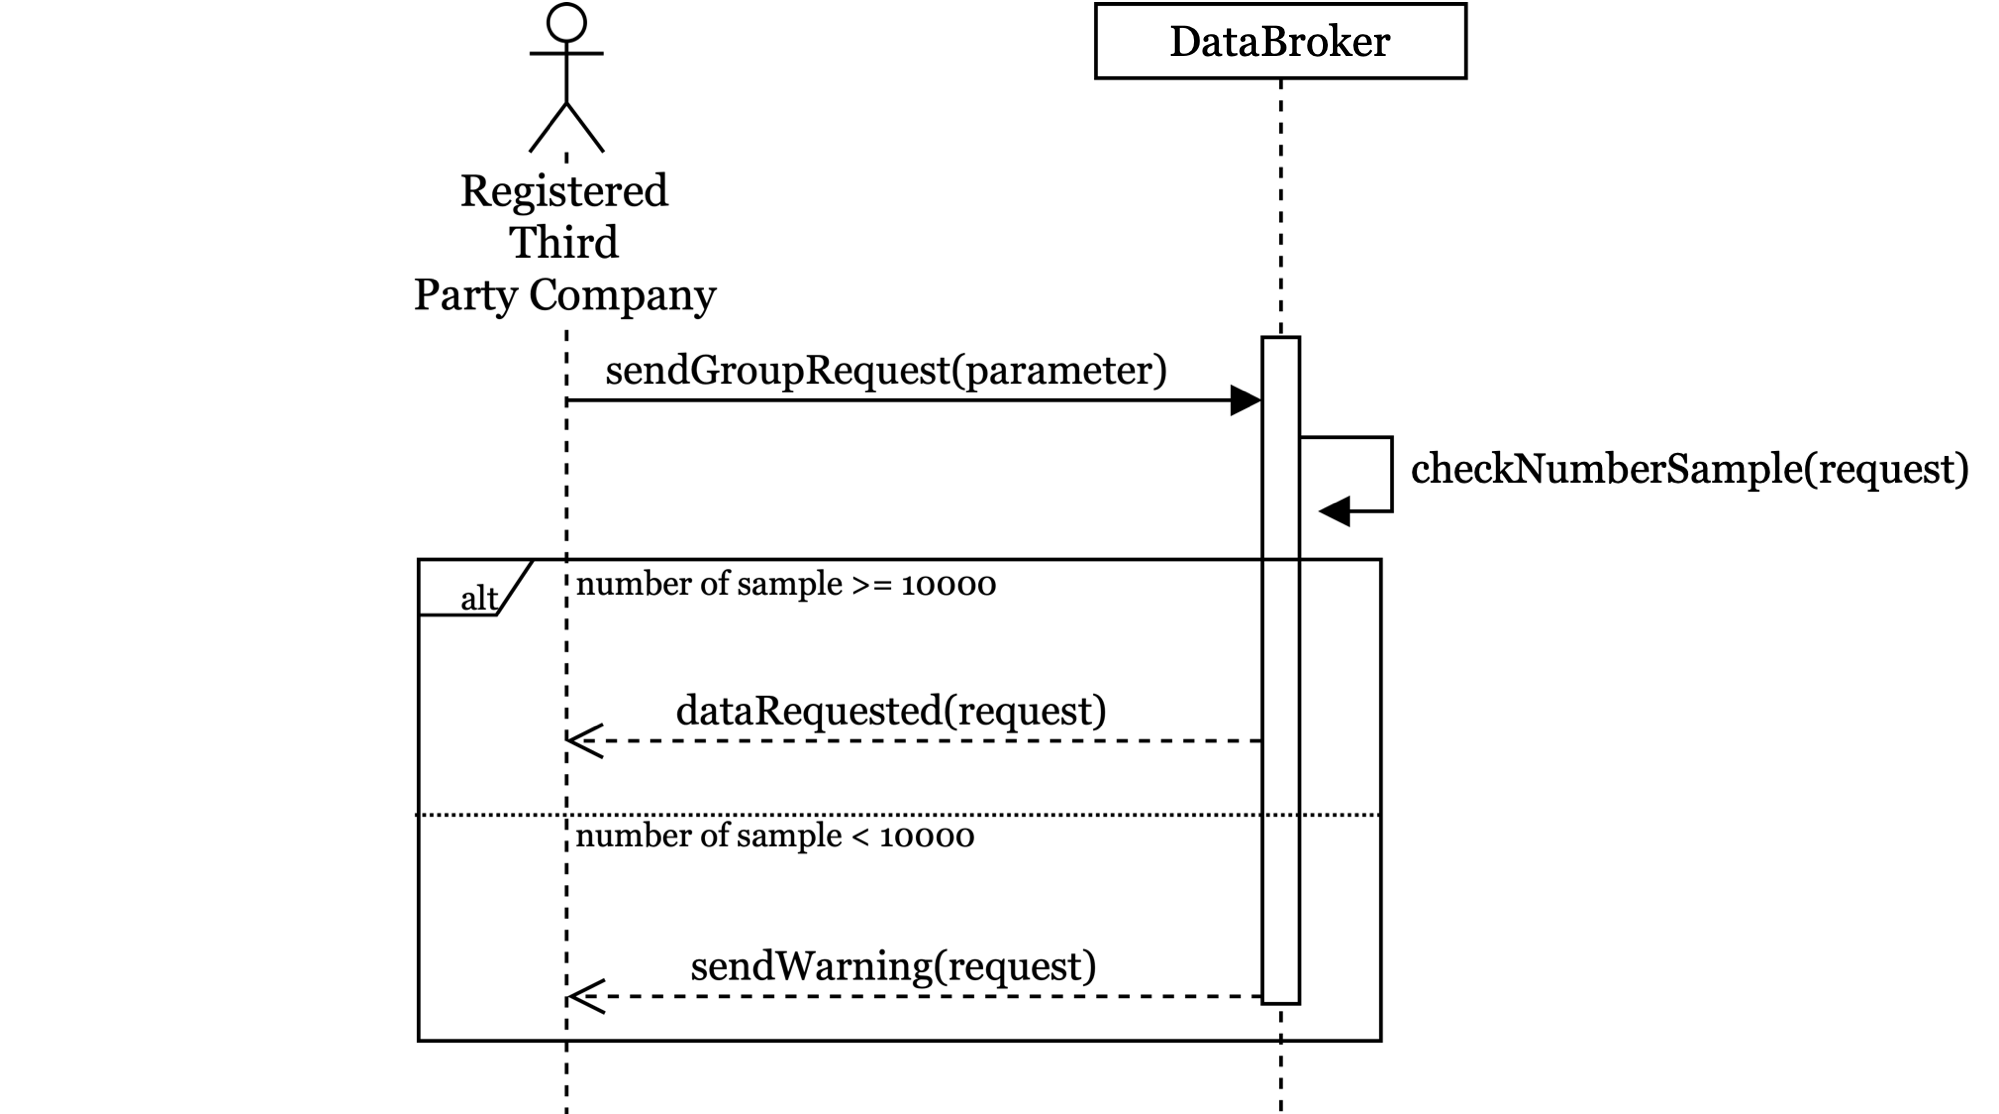
\includegraphics[scale=.3]{images/sequenceDiagram1.png}
			\caption{Sequence Diagram Scenario 1 \label{fig:Sequence Diagram Scenario 1}}
		\end{figure}
		\begin{minipage}{\textwidth}
			{\bf Scenario 2}
			\vspace{3mm}

			A hospital wants to monitor a convalescing patient who has been relesed. The patient has installed TrackMe, the ospital Using TrackMe's API sends to him a individual request data with the option of receiving new data as soon as the are available. The patient accepts the request so the ospital can monitor him.
			\vspace{5mm}
		\end{minipage}
		\begin{figure}[H]
			\centering
			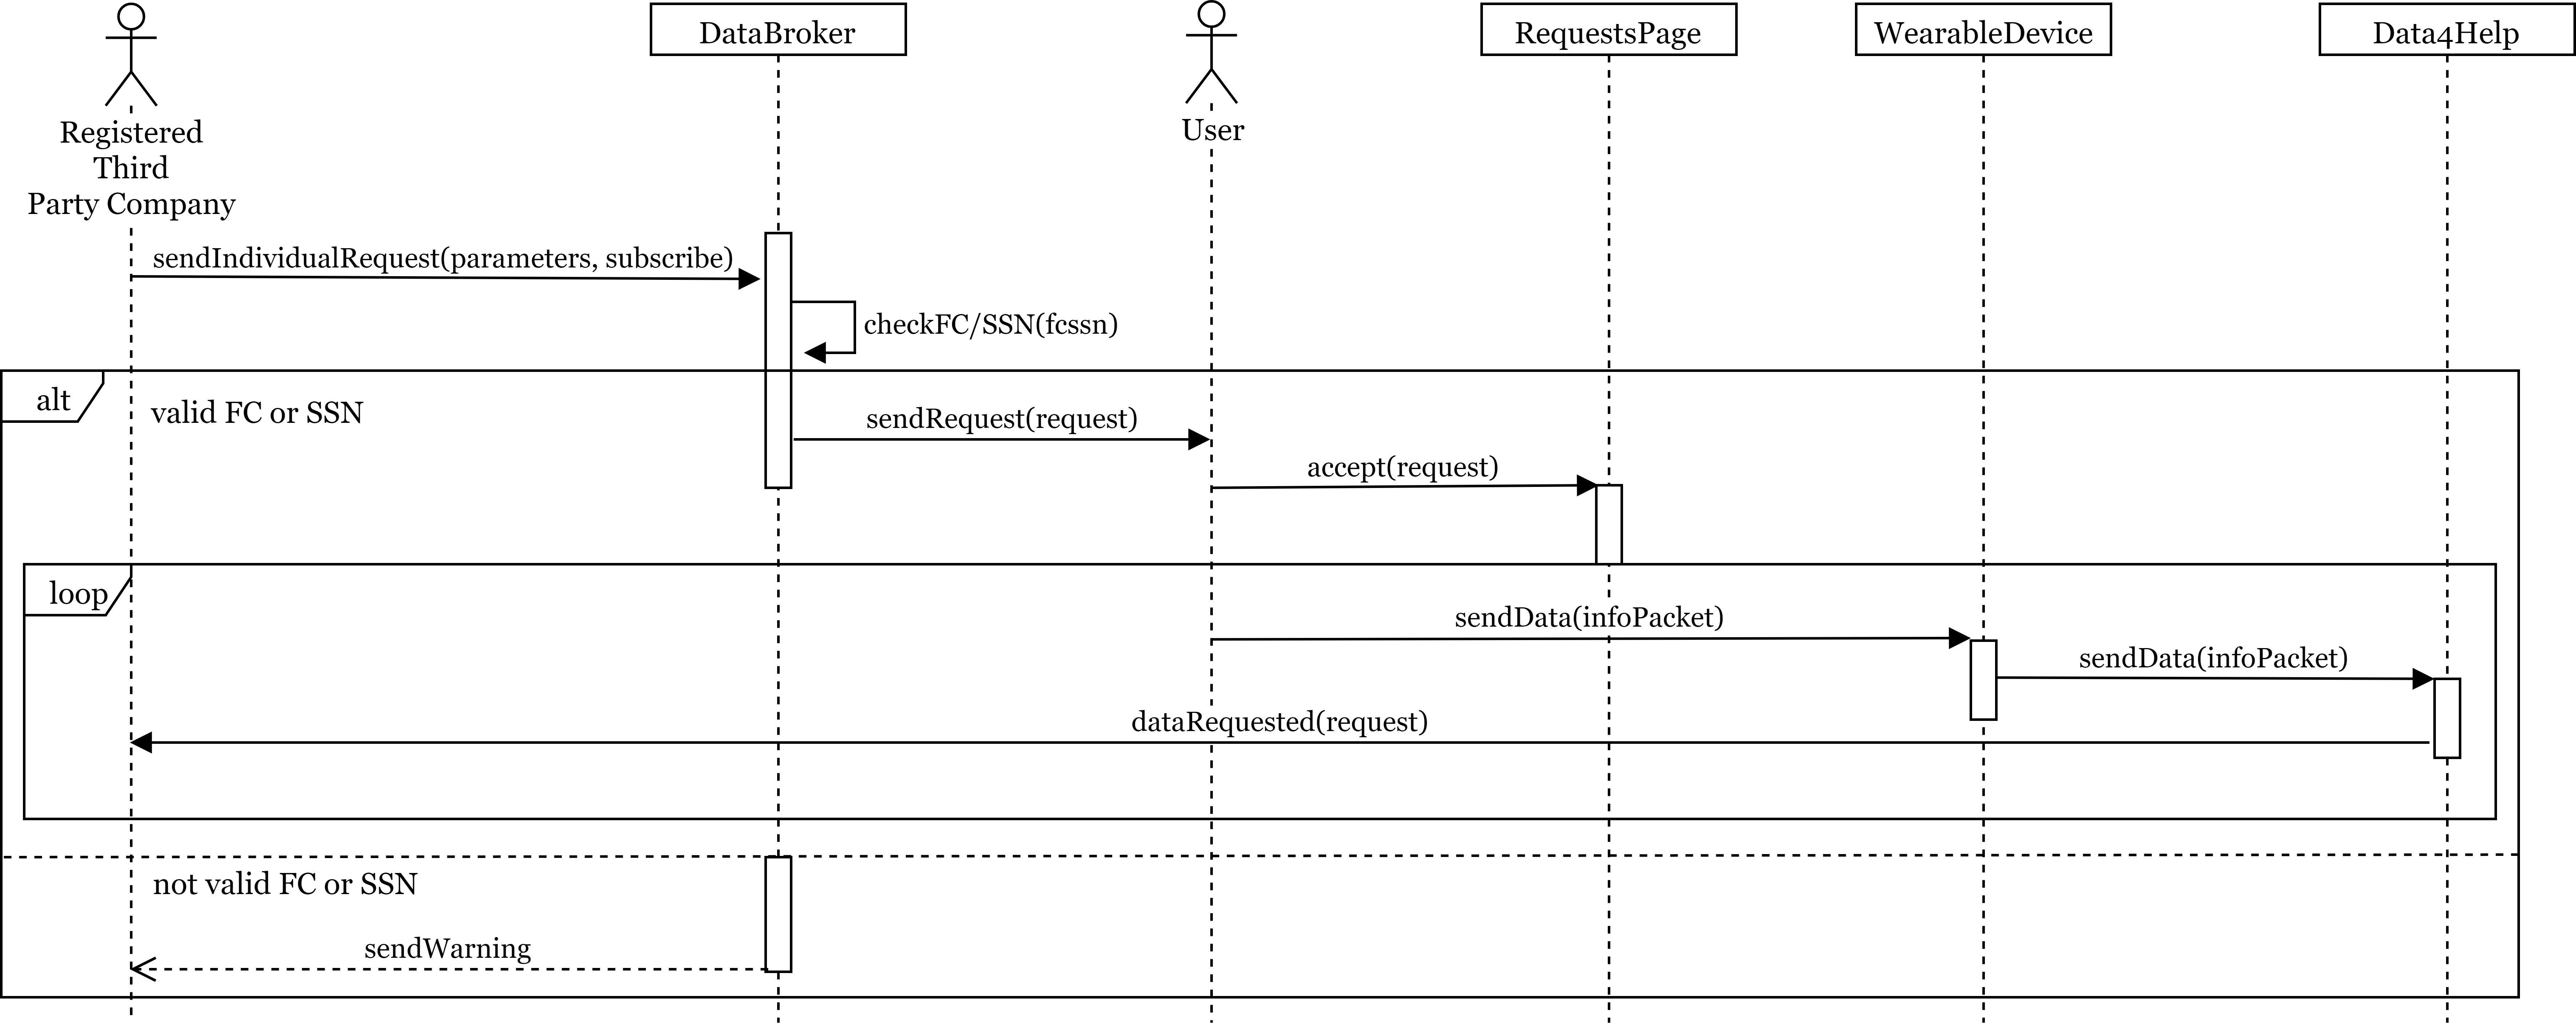
\includegraphics[scale=.05]{images/sequenceDiagram2.png}
			\caption{Sequence Diagram Scenario 2 \label{fig:Sequence Diagram Scenario 2}}
		\end{figure}
		\begin{minipage}{\textwidth}

		\end{minipage}
		\begin{minipage}[t]{\textwidth}
			{\bf Scenario 3}
			\vspace{3mm}

			Mrs. Jane is 75 years old. She always forgot to drink water and she eats very little. His son buy to her a smartwatch and install the TrackMe's application subscribing Jane to AutomatedSOS service. One day Jane feels bad due to an hypovolemia so her blood pressure drops dramatically. The smartwatch recognize that the value is under the minimum then an ambulance is called automatcally. Jane arrives to the hospital in time.

			\vspace{5mm}
		\end{minipage}
		\begin{figure}[H]
			\centering
			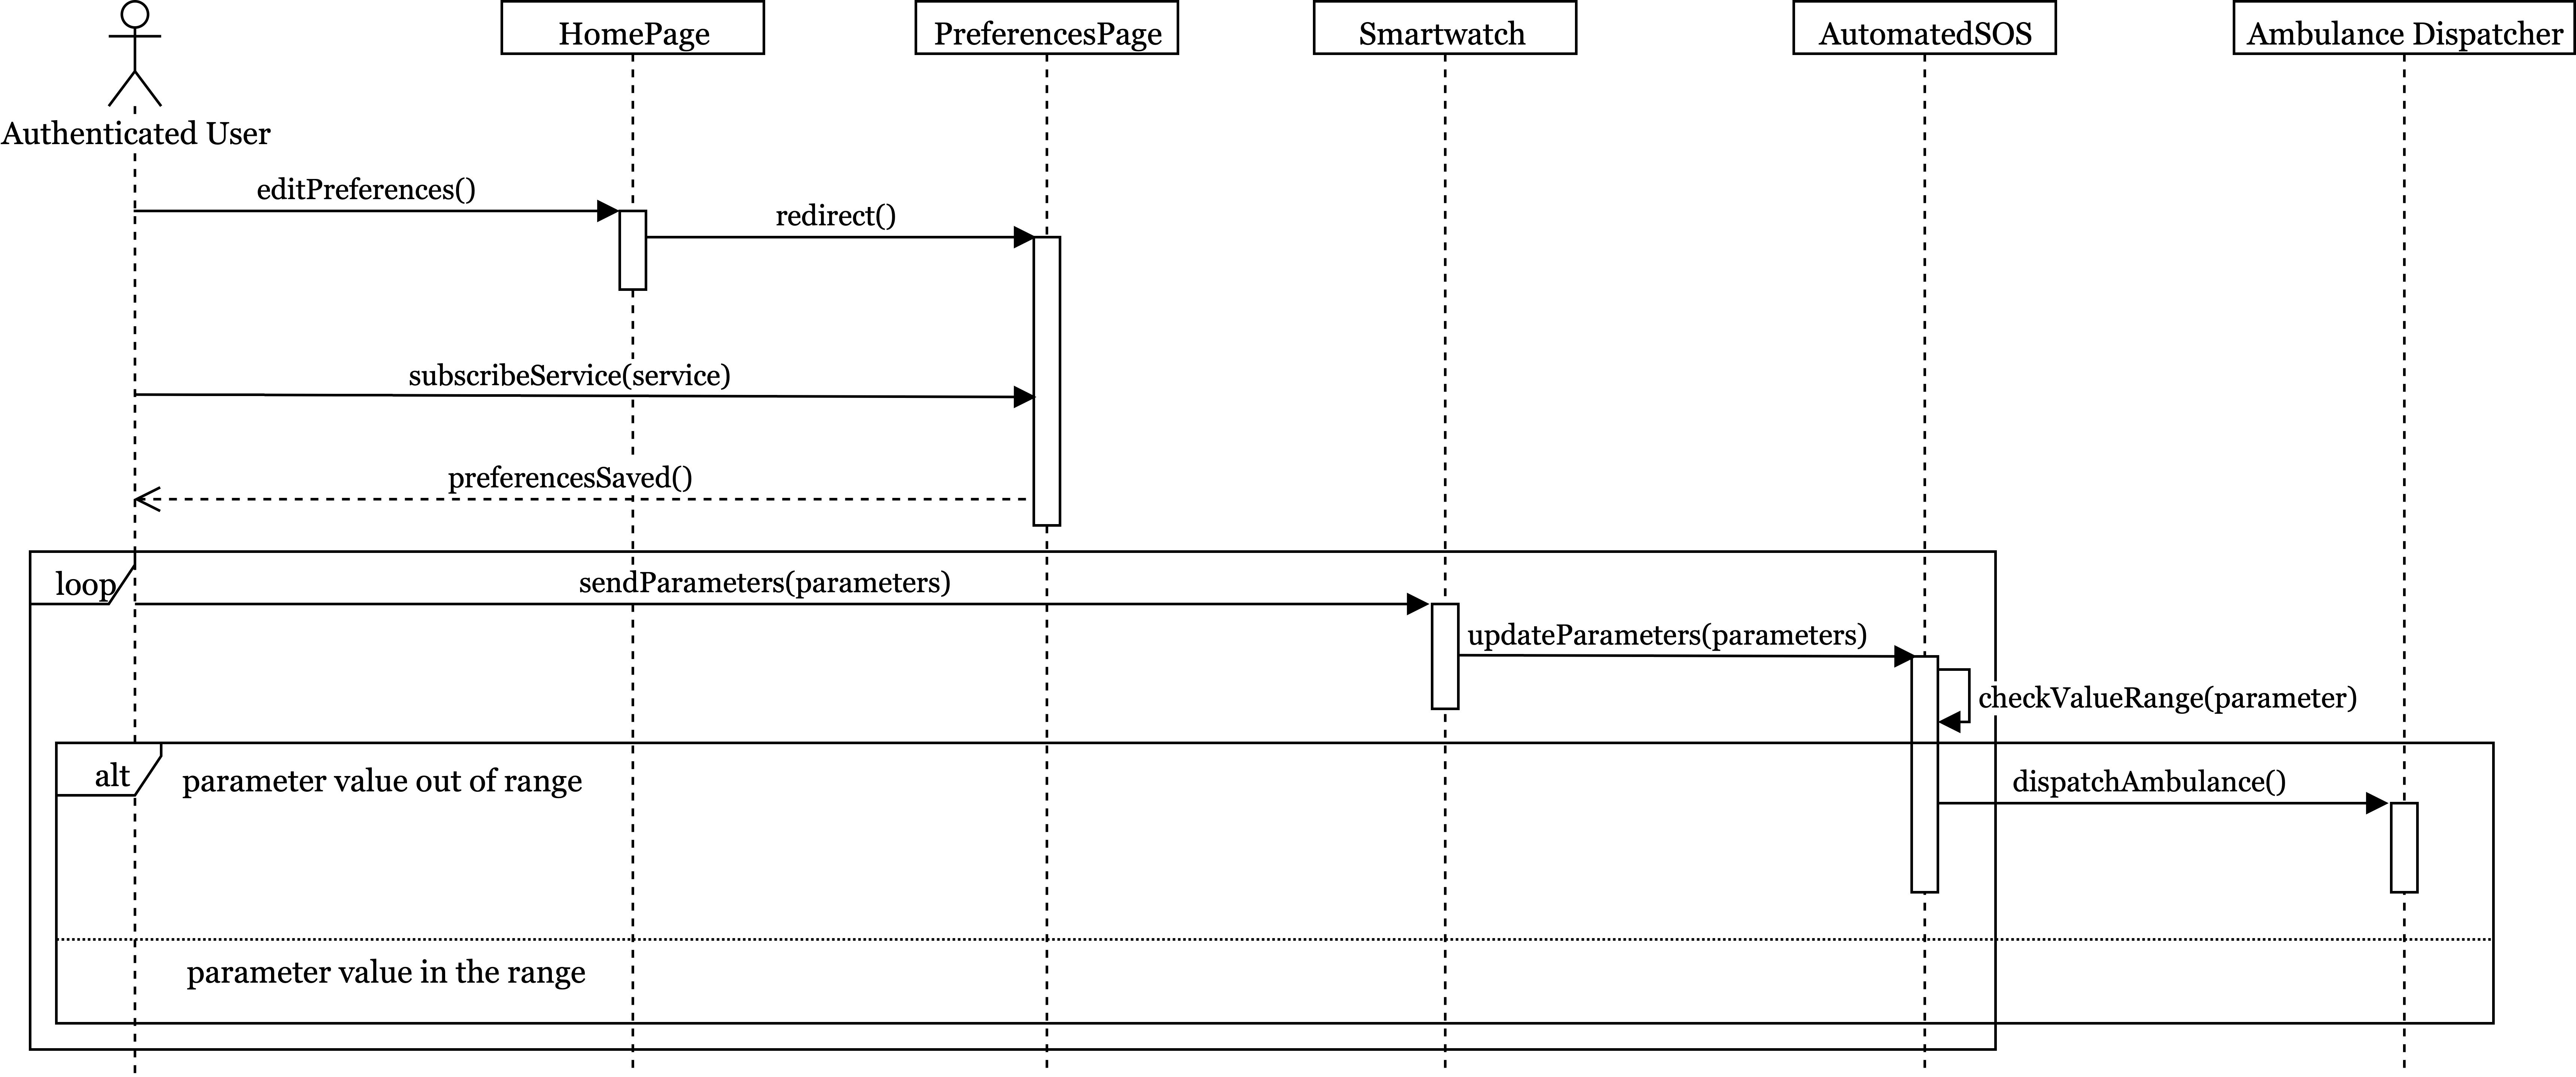
\includegraphics[scale=.05]{images/sequenceDiagram3.png}
			\caption{Sequence Diagram Scenario 3 \label{fig:Sequence Diagram Scenario 3}}
		\end{figure}
		\begin{minipage}{\textwidth}

		\end{minipage}
		\begin{minipage}{\textwidth}
			{\bf Scenario 4}
			\vspace{3mm}

			Mario wants to organize a running event in his city, he is subscribed to Track4Run so he opens the events page and creates a new one. He selects the route, date and time. The operation ends successfully so the event is organized but Mario realizes that he can't be present at the event. He edits the day of the event but due to another event already organized in the same place, date and time the editing operation fails. Mario finally decides to delete the event.

			\vspace{5mm}
		\end{minipage}
		\begin{figure}[H]
			\centering
			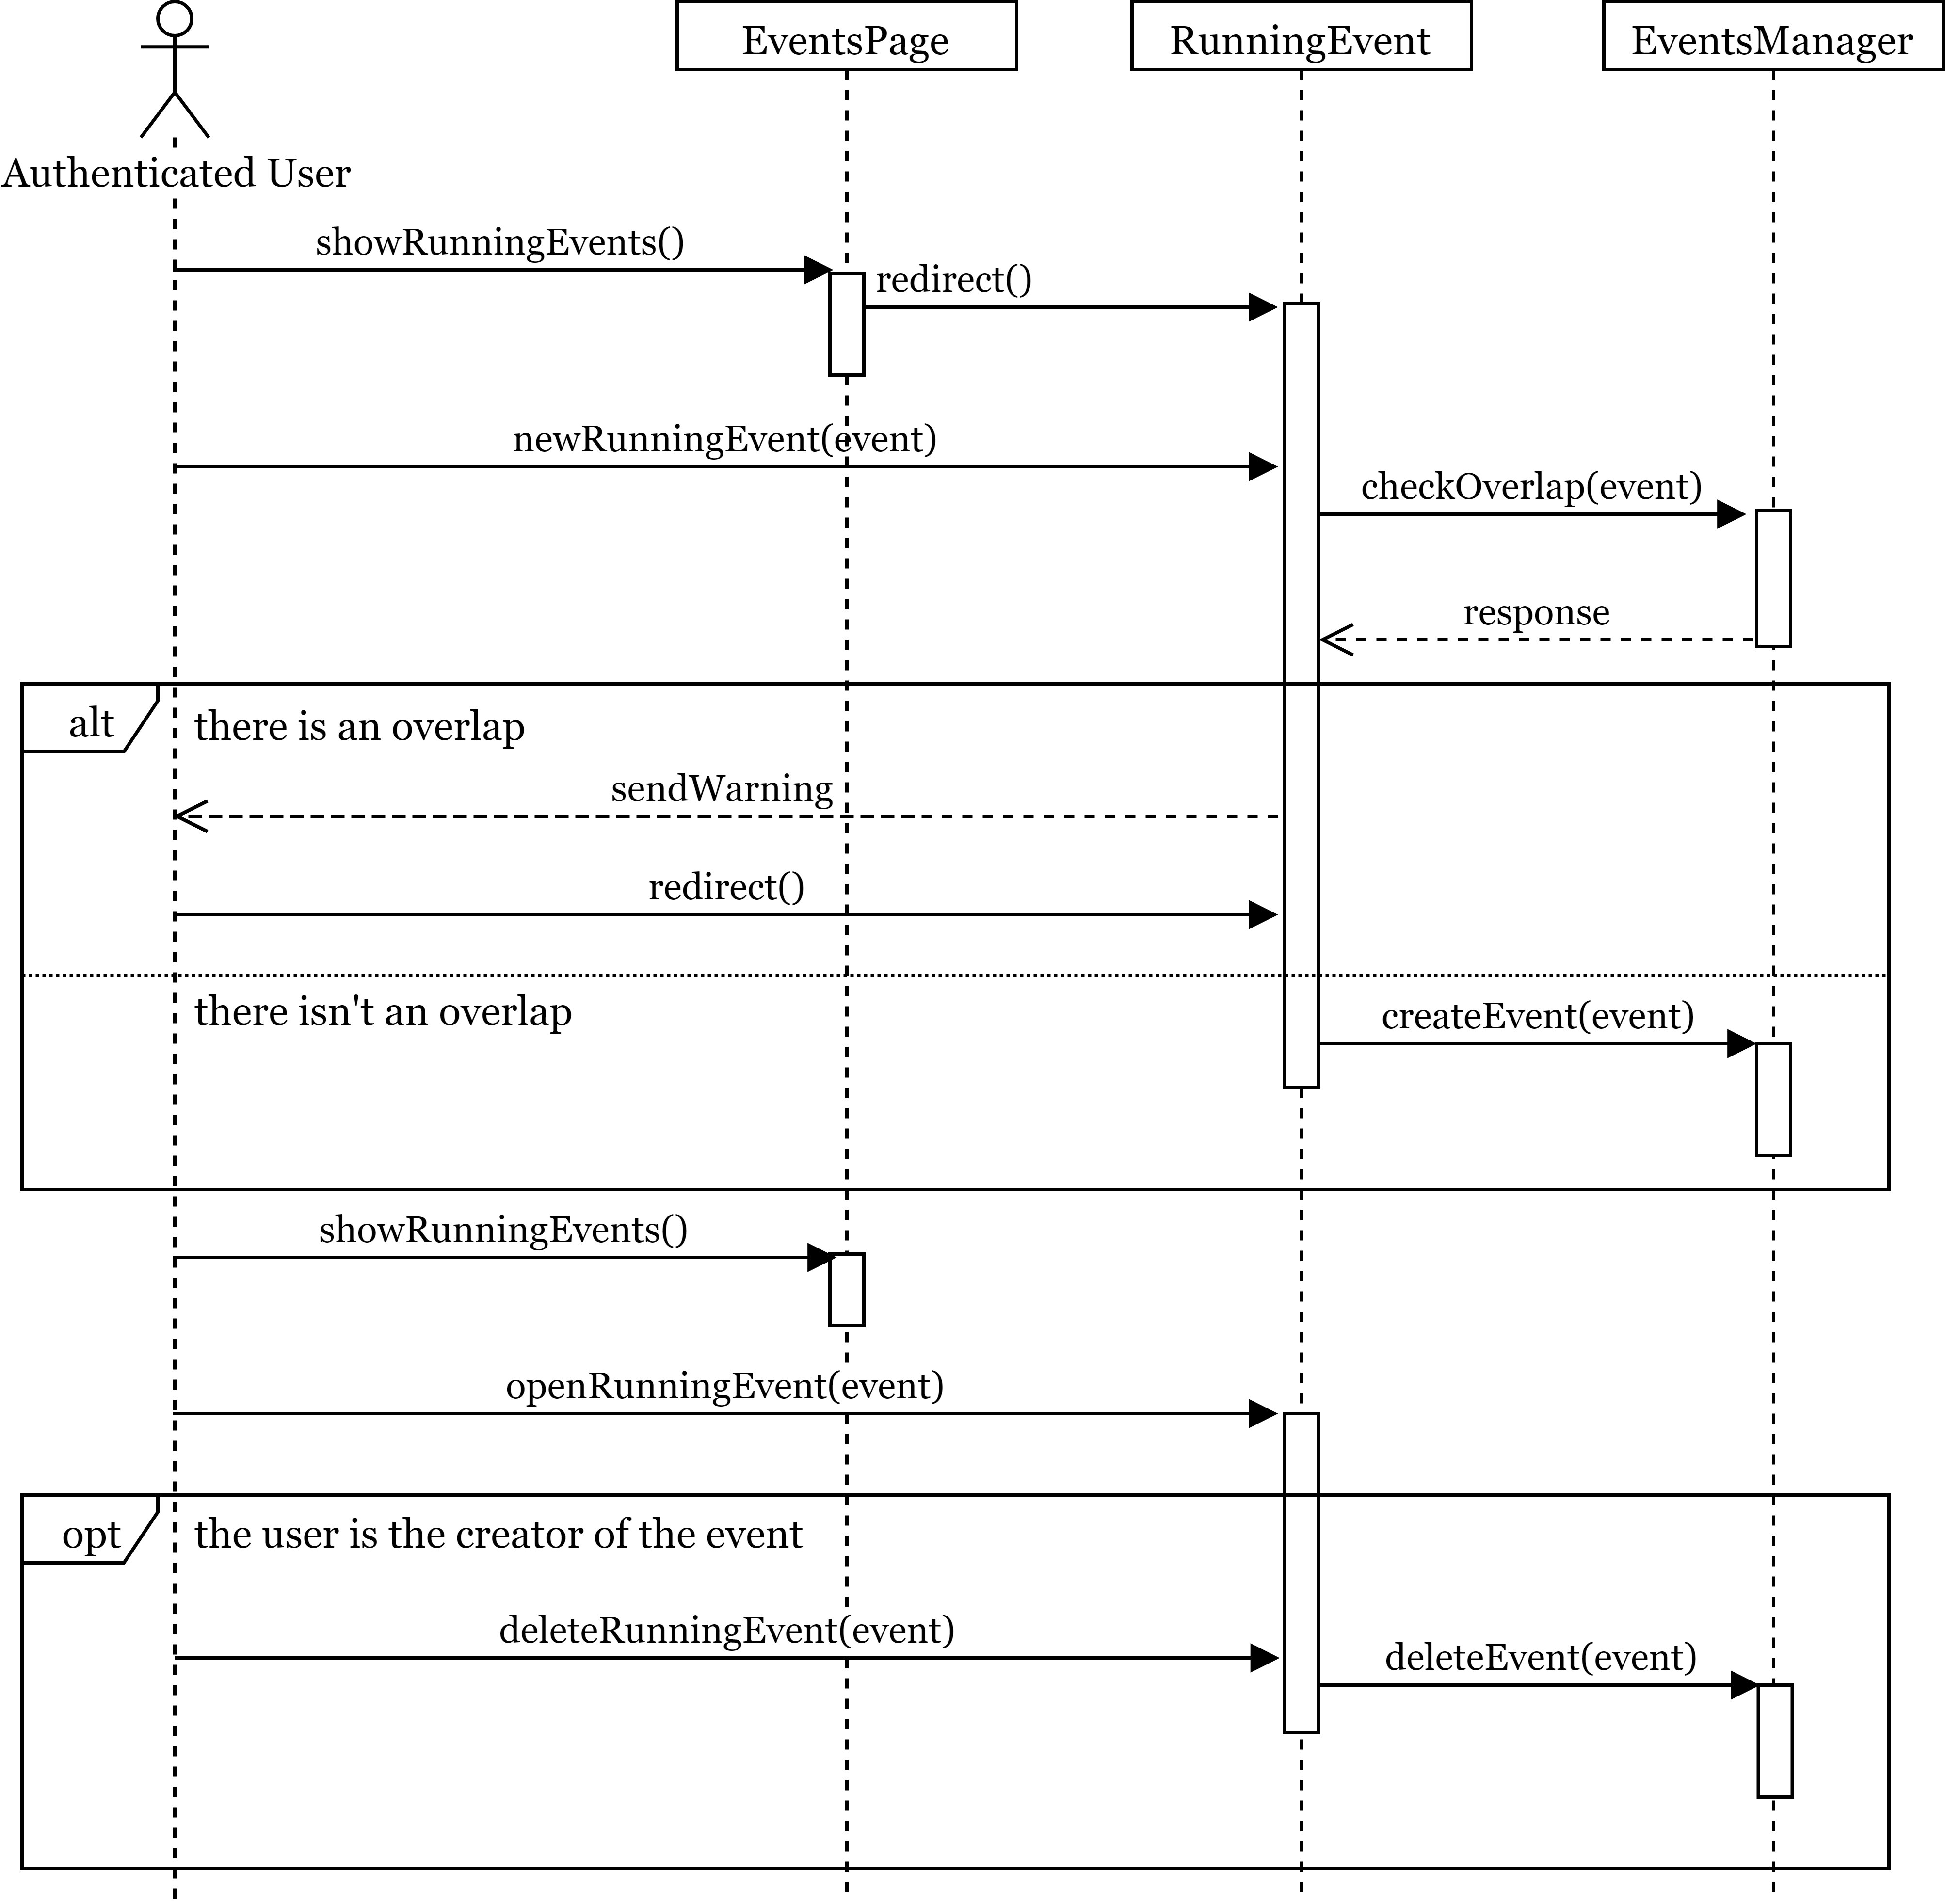
\includegraphics[scale=.07]{images/sequenceDiagram4.png}
			\caption{Sequence Diagram Scenario 4 \label{fig:Sequence Diagram Scenario 4}}
		\end{figure}
		\begin{minipage}{\textwidth}

		\end{minipage}
		\begin{minipage}{\textwidth}
			{\bf Scenario 5}
			\vspace{3mm}

			Anne runs for hobbies, she decides to subribe to Track4Run. She open the events page and she see one that interests her so she enrolls to it. She unfortunately breaks her foot so she can't participate but thanks to the option to see the map with the position of the participants she will at least be able to see the event progress.
			\vspace{5mm}
		\end{minipage}
		\begin{figure}[H]
			\centering
			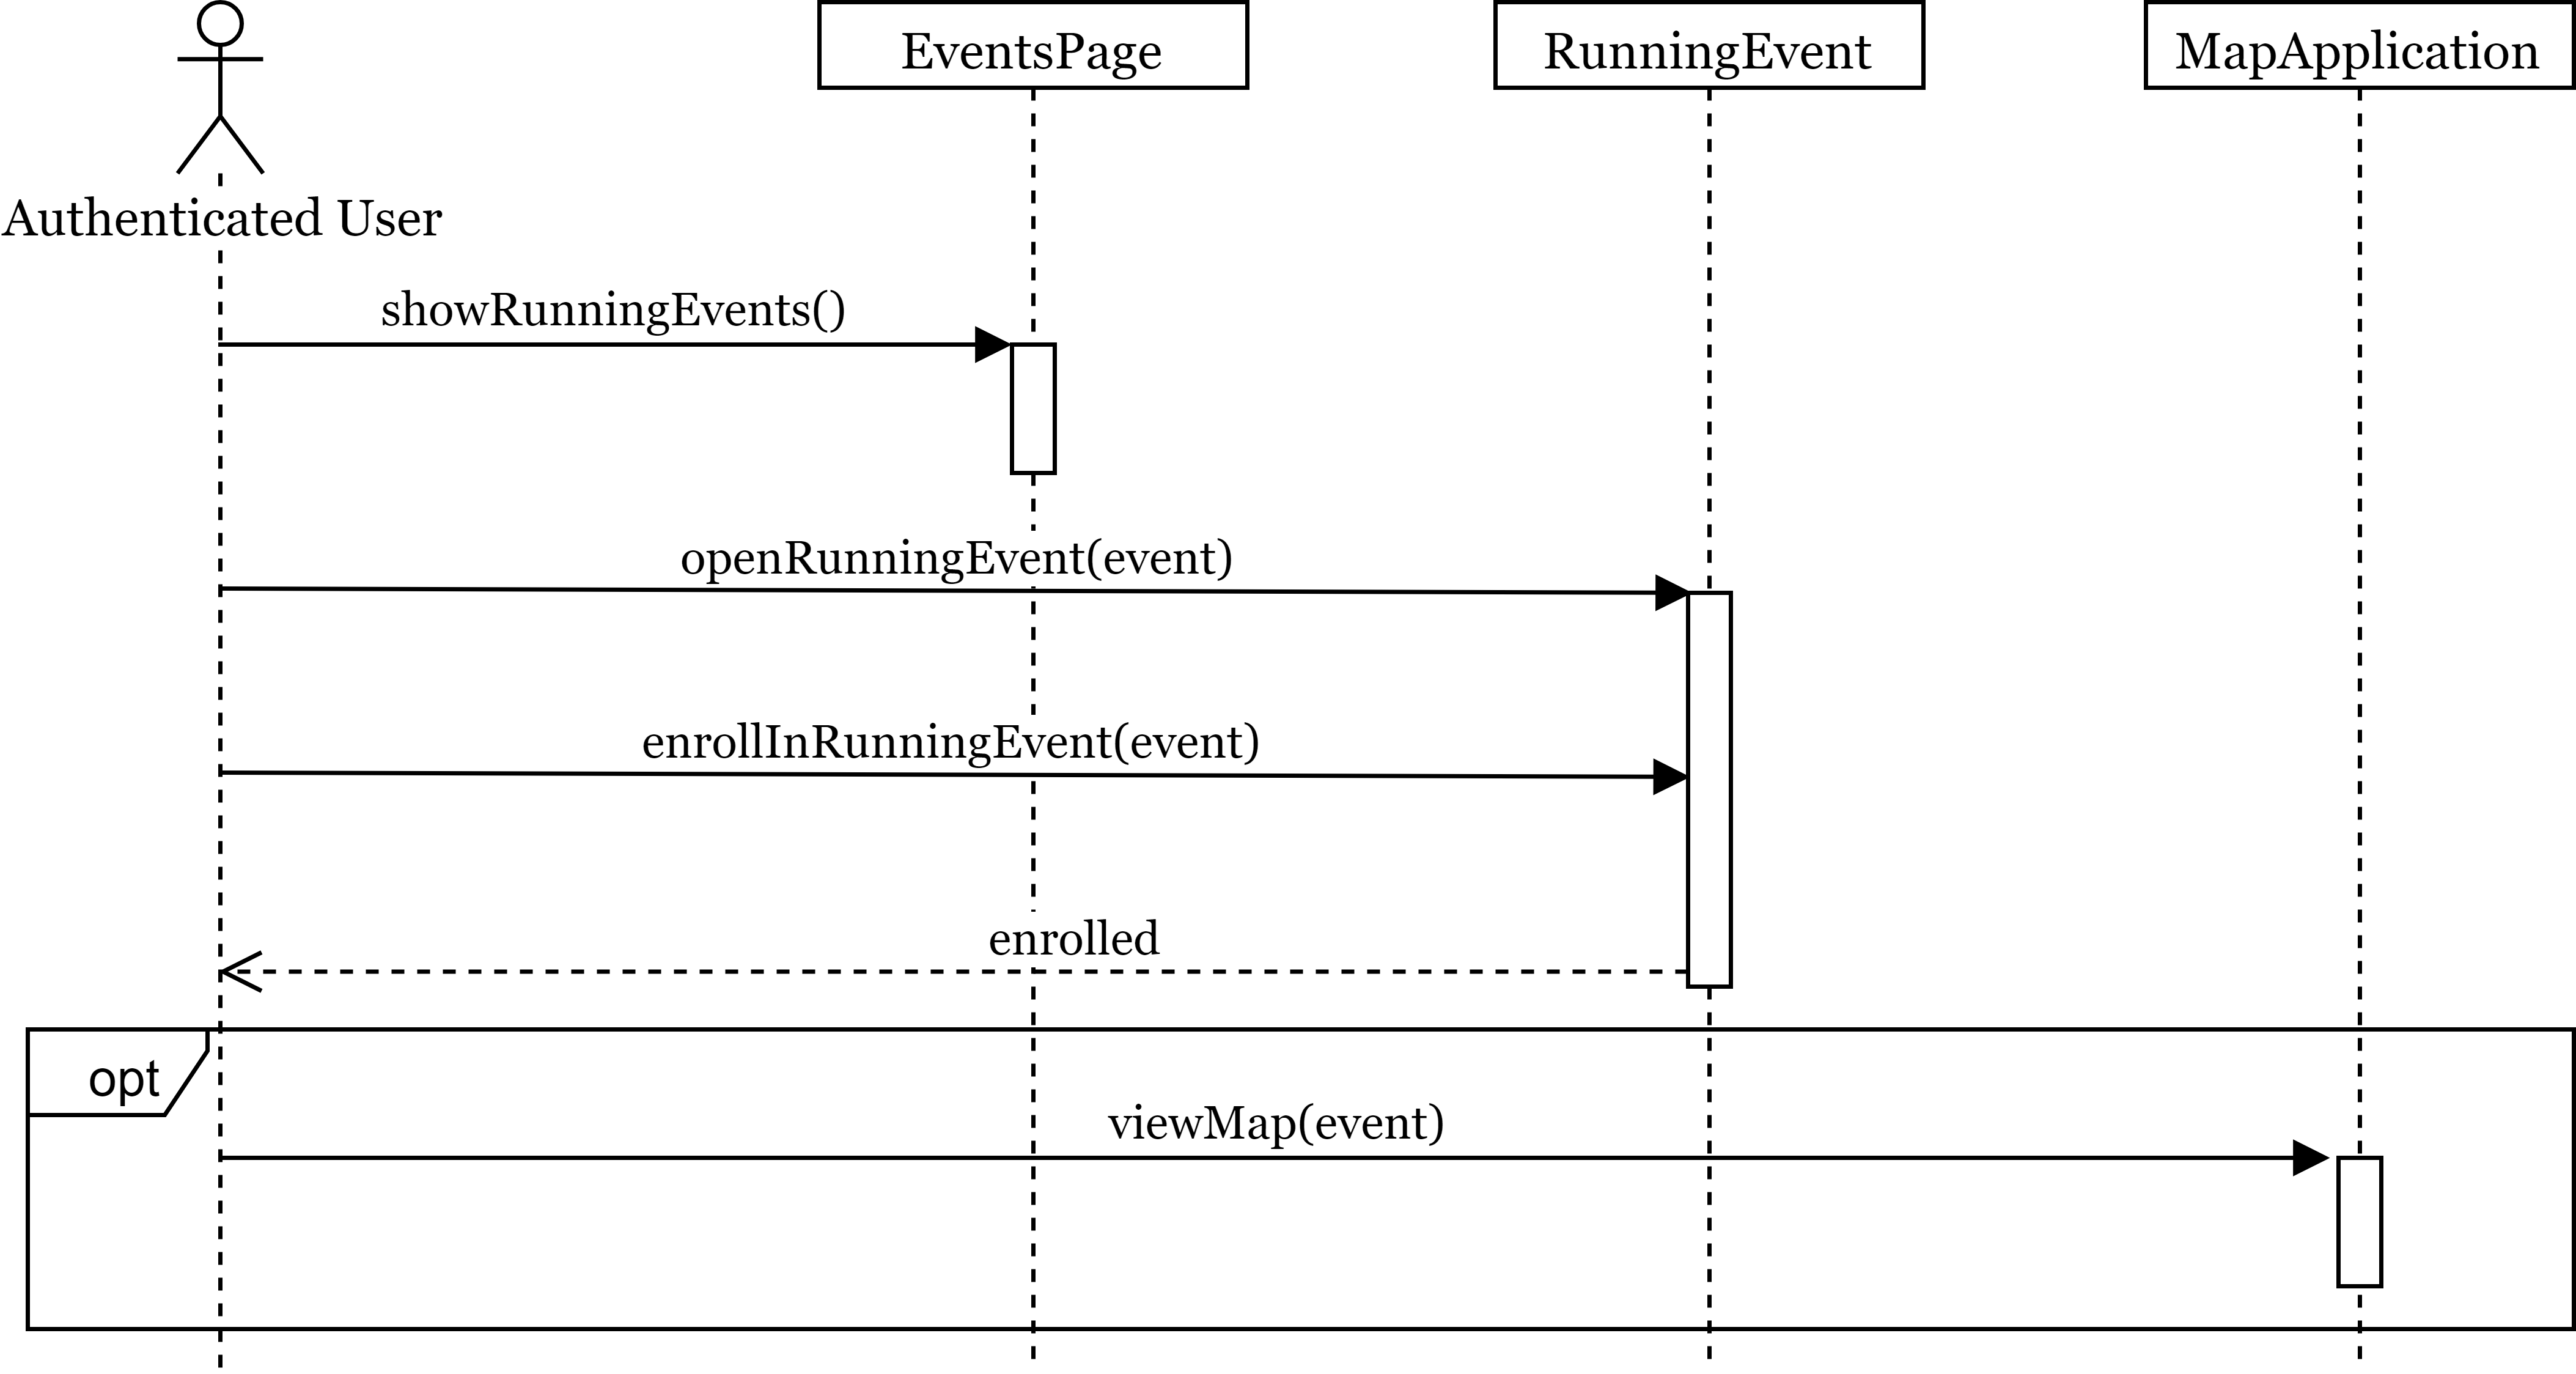
\includegraphics[scale=.08]{images/sequenceDiagram5.png}
			\caption{Sequence Diagram Scenario 5 \label{fig:Sequence Diagram Scenario 5}}
		\end{figure}


\subsection{Performance requirements}

Our system needs to permit a large number of third party companies to always operate on our services, and in the same way must promptly operate the incoming data from a large number of customers. It must therefore be scalable on the increasing number of users over time, and ready to serve at least 10.000 customers and 200 companies at launch.

The software on customer's device must be reactive, and must take into account communication protocols unreliability, transmitting all the data that wasn't succesfully sent after an occasional internet or bluetooth connection disservice.

\subsection{Design constraints}

\subsubsection{Standard compliance}

As per privacy policies, the system must ask appropriate permissions to be installed on the respective device, and must ask the customer to accept a statement that describes the use of the information we collect about him/her, at the moment of registering to our services.

\subsubsection{Hardware limitations}

Following are the hardware limitations required by the end customer for using our services.

\vspace*{8mm}
\begin{minipage}{\textwidth}
{\bf Wearable Device}
\begin{itemize}
	\item WearOS platform
	\item GPS
	\item Bluetooth Low Energy
	\item Heart rate sensor
	\item Blood pressure sensor
\end{itemize}
\end{minipage}

\vspace*{8mm}
\begin{minipage}{\textwidth}
{\bf Smartphone}
\begin{itemize}
	\item Android or iOS platform
	\item Bluetooth Low Energy
	\item Wi-Fi or 3G/4G technology
\end{itemize}
\end{minipage}

\subsection{Software system attributes}

\subsubsection{Reliability}
   AutomatedSOS it the critical component of the application, thus it's infrastracture should be characterized by the lowest MTTR possible.\\
   A larger MTTR is acceptable for our business to business components, however it's mandatory to prevent "data loss" (ie : using RAID configurations for servers)


\subsubsection{Availability}


	AutomatedSOS service must be up and running 24/7, the user must be quickly notified of
	any communication issues between smartphone and AutomatedSOS smartdevices or with Track4Help servers.\\
	Track4Run service should be operative only during day hours, we expect a low utilization of the service during night hours as shown
	in the histogram (Fig. 19).\\
	Companies and devices should be able to communicate with Track4Help servers 24/7.

\begin{figure}[H]
	\center
	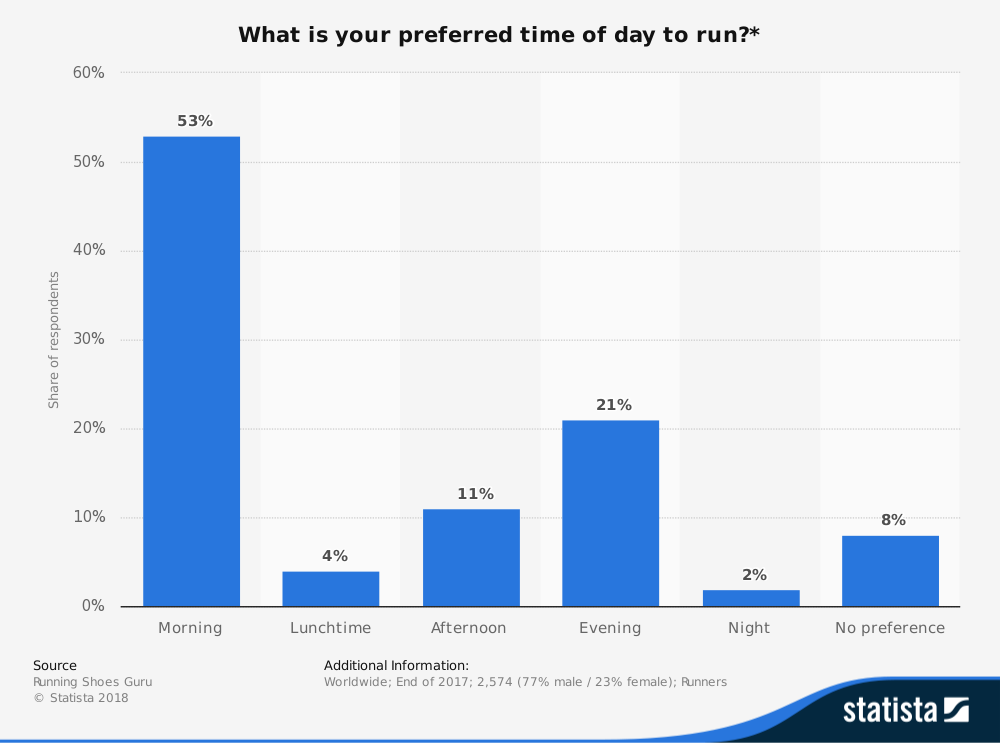
\includegraphics[scale=0.35]{images/statista_runhours.png}
	\caption{Preferred time of day for running (statista.com)}
\end{figure}

\subsubsection{Security}

In order to guarantee the protection of customer's sensible data, all internet traffic must be encrypted with SSL and sent through HTTPS protocol; also every end point of such data transfer that's in our control must verify the other side's certificate and reject any transmission if invalid.\\
All Bluetooth communication must be encrypted too.\\


\subsubsection{Mantainability}

The back-end system must be capable of sustaining maintenance operations on a copy, to be then deployed after being tested on all its functions, in order to guarantee no down-time for the critical functions.

Software that's on devices will be updated through the appropriate app store, as needed.

\subsubsection{Portability}

Our smartphone application must be available for Android and iOS platforms. Cross platform developing tools can be used to achieve this.

The wearable application must be available for the Android Wear/WearOS and watchOS platforms, as they currently are, and in the following years will probably be, the leading platforms for wearable devices.

\begin{figure}[H]
	\center
	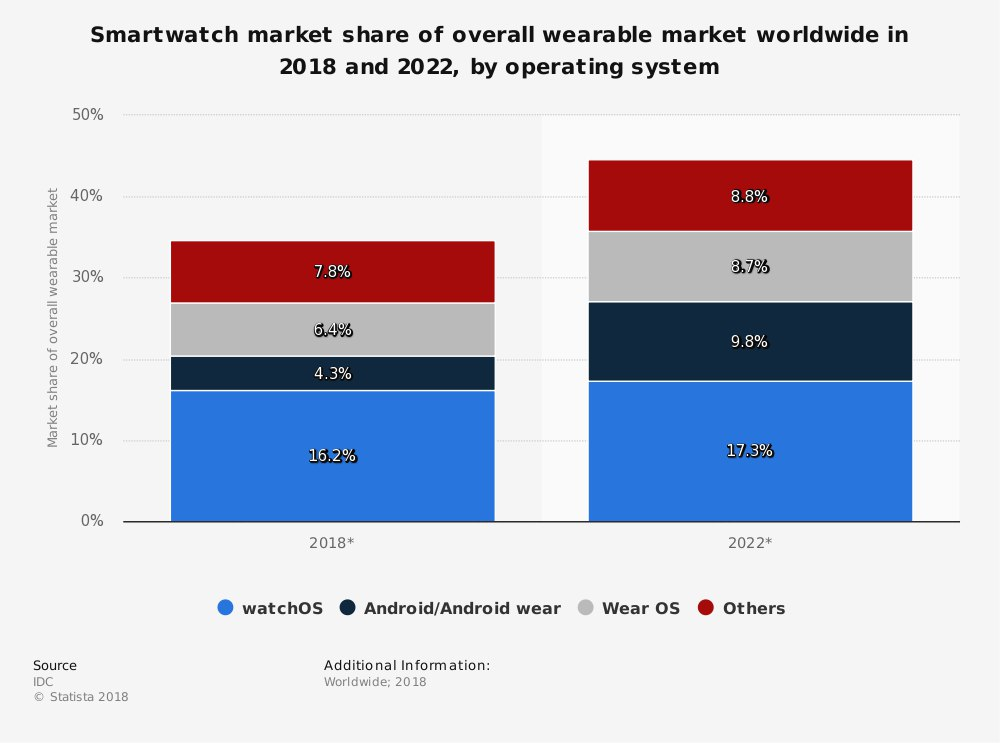
\includegraphics[scale=0.35]{images/statista_wearableOs.jpg}
	\caption{Leading operating systems for wearable devices (statista.com)}
\end{figure}

\end{document}
